\documentclass[]{article}
\usepackage{lmodern}
\usepackage{amssymb,amsmath}
\usepackage{ifxetex,ifluatex}
\usepackage{fixltx2e} % provides \textsubscript
\ifnum 0\ifxetex 1\fi\ifluatex 1\fi=0 % if pdftex
  \usepackage[T1]{fontenc}
  \usepackage[utf8]{inputenc}
\else % if luatex or xelatex
  \ifxetex
    \usepackage{mathspec}
  \else
    \usepackage{fontspec}
  \fi
  \defaultfontfeatures{Ligatures=TeX,Scale=MatchLowercase}
  \newcommand{\euro}{€}
\fi
% use upquote if available, for straight quotes in verbatim environments
\IfFileExists{upquote.sty}{\usepackage{upquote}}{}
% use microtype if available
\IfFileExists{microtype.sty}{%
\usepackage{microtype}
\UseMicrotypeSet[protrusion]{basicmath} % disable protrusion for tt fonts
}{}
\usepackage[margin=1in]{geometry}
\usepackage{hyperref}
\PassOptionsToPackage{usenames,dvipsnames}{color} % color is loaded by hyperref
\hypersetup{unicode=true,
            pdftitle={Statistical analysis},
            pdfborder={0 0 0},
            breaklinks=true}
\urlstyle{same}  % don't use monospace font for urls
\usepackage{longtable,booktabs}
\usepackage{graphicx,grffile}
\makeatletter
\def\maxwidth{\ifdim\Gin@nat@width>\linewidth\linewidth\else\Gin@nat@width\fi}
\def\maxheight{\ifdim\Gin@nat@height>\textheight\textheight\else\Gin@nat@height\fi}
\makeatother
% Scale images if necessary, so that they will not overflow the page
% margins by default, and it is still possible to overwrite the defaults
% using explicit options in \includegraphics[width, height, ...]{}
\setkeys{Gin}{width=\maxwidth,height=\maxheight,keepaspectratio}
\setlength{\parindent}{0pt}
\setlength{\parskip}{6pt plus 2pt minus 1pt}
\setlength{\emergencystretch}{3em}  % prevent overfull lines
\providecommand{\tightlist}{%
  \setlength{\itemsep}{0pt}\setlength{\parskip}{0pt}}
\setcounter{secnumdepth}{5}

%%% Use protect on footnotes to avoid problems with footnotes in titles
\let\rmarkdownfootnote\footnote%
\def\footnote{\protect\rmarkdownfootnote}

%%% Change title format to be more compact
\usepackage{titling}

% Create subtitle command for use in maketitle
\newcommand{\subtitle}[1]{
  \posttitle{
    \begin{center}\large#1\end{center}
    }
}

\setlength{\droptitle}{-2em}
  \title{Statistical analysis}
  \pretitle{\vspace{\droptitle}\centering\huge}
  \posttitle{\par}
  \author{}
  \preauthor{}\postauthor{}
  \date{}
  \predate{}\postdate{}



% Redefines (sub)paragraphs to behave more like sections
\ifx\paragraph\undefined\else
\let\oldparagraph\paragraph
\renewcommand{\paragraph}[1]{\oldparagraph{#1}\mbox{}}
\fi
\ifx\subparagraph\undefined\else
\let\oldsubparagraph\subparagraph
\renewcommand{\subparagraph}[1]{\oldsubparagraph{#1}\mbox{}}
\fi

\begin{document}
\maketitle

\section{Project Summary}\label{project-summary}

\textbf{Collaborators}

J.T. Lennon, \emph{Indiana University, Bloomington, IN}

S.W. Wilhelm, \emph{University of Tennessee - Knoxville, Knoxville TN}

\textbf{Project questions}

\begin{enumerate}
\def\labelenumi{\arabic{enumi}.}
\tightlist
\item
  Does resource stoichiometry affect the growth rate of
  \emph{Synechococcus}?
\item
  How does resource stoichiometry alter ecological dynamics?
\item
  Does stoichiometry alter phenotypic (co)evolution in cyanobacteria and
  phage?
\end{enumerate}

\textbf{Data collection}

Briefly, all data for this project was collected during a long term
continuous culture experimental evolution study with
\emph{Synechococcus} and SRIM-8 cyanomyophage.

For a complete description of the materials and methods for this
repository, see Larsen \emph{et al.} 2016.

Funding for this project was provided in part by the National Science
Foundation, Michigan State University BEACON Center for Evolution in
Action, and Indiana University.

\newpage

\tableofcontents
\newpage

\section{\texorpdfstring{Physiological growth: Does nutrient
stoichiometry affect the growth rate of
\emph{Synechococcus}?}{Physiological growth: Does nutrient stoichiometry affect the growth rate of Synechococcus?}}\label{physiological-growth-does-nutrient-stoichiometry-affect-the-growth-rate-of-synechococcus}

\textbf{Overview}: In this experiment, we tested for growth enhancement
with the addtion of N or P to our stoichiometrically amended AN media
(Lennon \emph{et al.} 2007; see Larsen \emph{et al.} 2016 Table S1).

\subsection{Summary of Major Results}\label{summary-of-major-results}

\begin{enumerate}
\def\labelenumi{\arabic{enumi}.}
\tightlist
\item
  Addition of N or P to our N-limited or P-limited media increased
  \emph{Synechococcus} in comparison to the control treatment (Figure 1,
  Table 1).
\end{enumerate}

*Analysis \url{Notes:*}

\begin{enumerate}
\def\labelenumi{\arabic{enumi}.}
\tightlist
\item
  Population growth curve data was collected on a Biotek Synergy Mx
  instrument loaded with softward version 2.01.12.
\item
  Growth rate calculations were completed using lab generated code for
  bacterial growth rate analysis for the above instrument and can be
  found at \texttt{http://github.com/LennonLab/Growth\_Curves}.
\end{enumerate}

\newpage

\subsection{\texorpdfstring{\emph{Synechococcus} growth rates with
response to nutrient
addition}{Synechococcus growth rates with response to nutrient addition}}\label{synechococcus-growth-rates-with-response-to-nutrient-addition}

\begin{figure}[htbp]
\centering
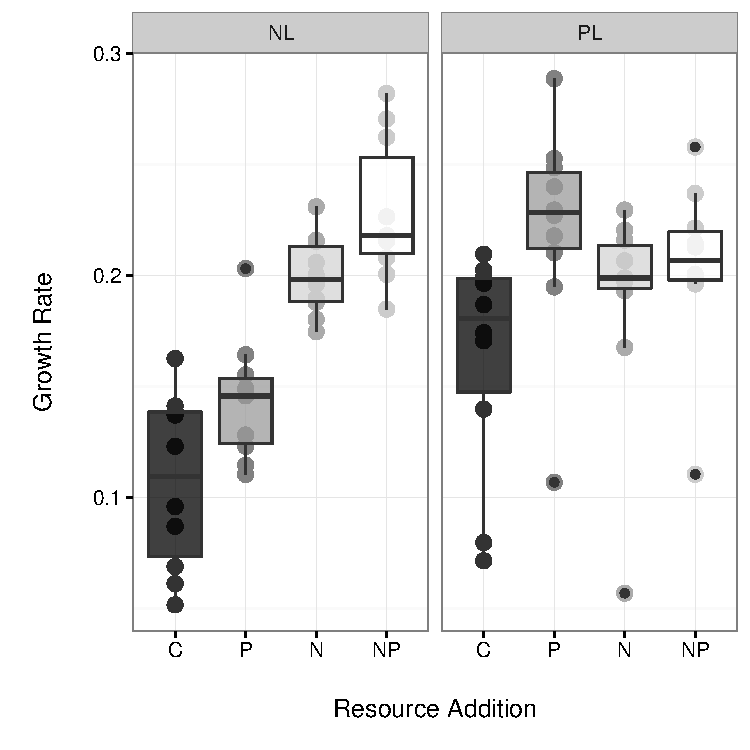
\includegraphics{analysis_ecoevostoich_files/figure-latex/gr-vis-1.pdf}
\caption{Nitrogen (N), phosphorus (P), or NP addition to the base
N-limited and P-limited media used in the chemostat experiment. Culture
controls (C) did not contain additional N or P.}
\end{figure}

\newpage

\subsubsection{Growth rate ANOVA tables}\label{growth-rate-anova-tables}

\textbf{N-limited}

\begin{longtable}[]{@{}cccccc@{}}
\caption{ANOVA table for NL nutrient addition}\tabularnewline
\toprule
\begin{minipage}[b]{0.19\columnwidth}\centering\strut
~
\strut\end{minipage} &
\begin{minipage}[b]{0.06\columnwidth}\centering\strut
Df
\strut\end{minipage} &
\begin{minipage}[b]{0.10\columnwidth}\centering\strut
Sum Sq
\strut\end{minipage} &
\begin{minipage}[b]{0.12\columnwidth}\centering\strut
Mean Sq
\strut\end{minipage} &
\begin{minipage}[b]{0.12\columnwidth}\centering\strut
F value
\strut\end{minipage} &
\begin{minipage}[b]{0.12\columnwidth}\centering\strut
Pr(\textgreater{}F)
\strut\end{minipage}\tabularnewline
\midrule
\endfirsthead
\toprule
\begin{minipage}[b]{0.19\columnwidth}\centering\strut
~
\strut\end{minipage} &
\begin{minipage}[b]{0.06\columnwidth}\centering\strut
Df
\strut\end{minipage} &
\begin{minipage}[b]{0.10\columnwidth}\centering\strut
Sum Sq
\strut\end{minipage} &
\begin{minipage}[b]{0.12\columnwidth}\centering\strut
Mean Sq
\strut\end{minipage} &
\begin{minipage}[b]{0.12\columnwidth}\centering\strut
F value
\strut\end{minipage} &
\begin{minipage}[b]{0.12\columnwidth}\centering\strut
Pr(\textgreater{}F)
\strut\end{minipage}\tabularnewline
\midrule
\endhead
\begin{minipage}[t]{0.19\columnwidth}\centering\strut
\textbf{med.add}
\strut\end{minipage} &
\begin{minipage}[t]{0.06\columnwidth}\centering\strut
3
\strut\end{minipage} &
\begin{minipage}[t]{0.10\columnwidth}\centering\strut
0.08993
\strut\end{minipage} &
\begin{minipage}[t]{0.12\columnwidth}\centering\strut
0.02998
\strut\end{minipage} &
\begin{minipage}[t]{0.12\columnwidth}\centering\strut
33.3
\strut\end{minipage} &
\begin{minipage}[t]{0.12\columnwidth}\centering\strut
1.743e-10
\strut\end{minipage}\tabularnewline
\begin{minipage}[t]{0.19\columnwidth}\centering\strut
\textbf{Residuals}
\strut\end{minipage} &
\begin{minipage}[t]{0.06\columnwidth}\centering\strut
36
\strut\end{minipage} &
\begin{minipage}[t]{0.10\columnwidth}\centering\strut
0.0324
\strut\end{minipage} &
\begin{minipage}[t]{0.12\columnwidth}\centering\strut
0.0009001
\strut\end{minipage} &
\begin{minipage}[t]{0.12\columnwidth}\centering\strut
NA
\strut\end{minipage} &
\begin{minipage}[t]{0.12\columnwidth}\centering\strut
NA
\strut\end{minipage}\tabularnewline
\bottomrule
\end{longtable}

\begin{longtable}[]{@{}ccccc@{}}
\caption{Posthoc comparisons using Tukey HSD}\tabularnewline
\toprule
\begin{minipage}[b]{0.13\columnwidth}\centering\strut
~
\strut\end{minipage} &
\begin{minipage}[b]{0.16\columnwidth}\centering\strut
diff
\strut\end{minipage} &
\begin{minipage}[b]{0.16\columnwidth}\centering\strut
lwr
\strut\end{minipage} &
\begin{minipage}[b]{0.16\columnwidth}\centering\strut
upr
\strut\end{minipage} &
\begin{minipage}[b]{0.16\columnwidth}\centering\strut
p adj
\strut\end{minipage}\tabularnewline
\midrule
\endfirsthead
\toprule
\begin{minipage}[b]{0.13\columnwidth}\centering\strut
~
\strut\end{minipage} &
\begin{minipage}[b]{0.16\columnwidth}\centering\strut
diff
\strut\end{minipage} &
\begin{minipage}[b]{0.16\columnwidth}\centering\strut
lwr
\strut\end{minipage} &
\begin{minipage}[b]{0.16\columnwidth}\centering\strut
upr
\strut\end{minipage} &
\begin{minipage}[b]{0.16\columnwidth}\centering\strut
p adj
\strut\end{minipage}\tabularnewline
\midrule
\endhead
\begin{minipage}[t]{0.13\columnwidth}\centering\strut
\textbf{N-C}
\strut\end{minipage} &
\begin{minipage}[t]{0.16\columnwidth}\centering\strut
\textbf{0.0929}
\strut\end{minipage} &
\begin{minipage}[t]{0.16\columnwidth}\centering\strut
\textbf{0.05677}
\strut\end{minipage} &
\begin{minipage}[t]{0.16\columnwidth}\centering\strut
\textbf{0.129}
\strut\end{minipage} &
\begin{minipage}[t]{0.16\columnwidth}\centering\strut
\textbf{2.426e-07}
\strut\end{minipage}\tabularnewline
\begin{minipage}[t]{0.13\columnwidth}\centering\strut
\textbf{NP-C}
\strut\end{minipage} &
\begin{minipage}[t]{0.16\columnwidth}\centering\strut
\textbf{0.1218}
\strut\end{minipage} &
\begin{minipage}[t]{0.16\columnwidth}\centering\strut
\textbf{0.0857}
\strut\end{minipage} &
\begin{minipage}[t]{0.16\columnwidth}\centering\strut
\textbf{0.158}
\strut\end{minipage} &
\begin{minipage}[t]{0.16\columnwidth}\centering\strut
\textbf{4.542e-10}
\strut\end{minipage}\tabularnewline
\begin{minipage}[t]{0.13\columnwidth}\centering\strut
\textbf{P-C}
\strut\end{minipage} &
\begin{minipage}[t]{0.16\columnwidth}\centering\strut
\textbf{0.03716}
\strut\end{minipage} &
\begin{minipage}[t]{0.16\columnwidth}\centering\strut
\textbf{0.001027}
\strut\end{minipage} &
\begin{minipage}[t]{0.16\columnwidth}\centering\strut
\textbf{0.0733}
\strut\end{minipage} &
\begin{minipage}[t]{0.16\columnwidth}\centering\strut
\textbf{0.04188}
\strut\end{minipage}\tabularnewline
\begin{minipage}[t]{0.13\columnwidth}\centering\strut
\textbf{NP-N}
\strut\end{minipage} &
\begin{minipage}[t]{0.16\columnwidth}\centering\strut
0.02893
\strut\end{minipage} &
\begin{minipage}[t]{0.16\columnwidth}\centering\strut
-0.007204
\strut\end{minipage} &
\begin{minipage}[t]{0.16\columnwidth}\centering\strut
0.06507
\strut\end{minipage} &
\begin{minipage}[t]{0.16\columnwidth}\centering\strut
0.1551
\strut\end{minipage}\tabularnewline
\begin{minipage}[t]{0.13\columnwidth}\centering\strut
\textbf{P-N}
\strut\end{minipage} &
\begin{minipage}[t]{0.16\columnwidth}\centering\strut
\textbf{-0.05574}
\strut\end{minipage} &
\begin{minipage}[t]{0.16\columnwidth}\centering\strut
\textbf{-0.09188}
\strut\end{minipage} &
\begin{minipage}[t]{0.16\columnwidth}\centering\strut
\textbf{-0.01961}
\strut\end{minipage} &
\begin{minipage}[t]{0.16\columnwidth}\centering\strut
\textbf{0.001056}
\strut\end{minipage}\tabularnewline
\begin{minipage}[t]{0.13\columnwidth}\centering\strut
\textbf{P-NP}
\strut\end{minipage} &
\begin{minipage}[t]{0.16\columnwidth}\centering\strut
\textbf{-0.08467}
\strut\end{minipage} &
\begin{minipage}[t]{0.16\columnwidth}\centering\strut
\textbf{-0.1208}
\strut\end{minipage} &
\begin{minipage}[t]{0.16\columnwidth}\centering\strut
\textbf{-0.04854}
\strut\end{minipage} &
\begin{minipage}[t]{0.16\columnwidth}\centering\strut
\textbf{1.564e-06}
\strut\end{minipage}\tabularnewline
\bottomrule
\end{longtable}

\textbf{P-limited}

\begin{longtable}[]{@{}cccccc@{}}
\caption{ANOVA table for PL nutrient addition}\tabularnewline
\toprule
\begin{minipage}[b]{0.19\columnwidth}\centering\strut
~
\strut\end{minipage} &
\begin{minipage}[b]{0.06\columnwidth}\centering\strut
Df
\strut\end{minipage} &
\begin{minipage}[b]{0.10\columnwidth}\centering\strut
Sum Sq
\strut\end{minipage} &
\begin{minipage}[b]{0.12\columnwidth}\centering\strut
Mean Sq
\strut\end{minipage} &
\begin{minipage}[b]{0.12\columnwidth}\centering\strut
F value
\strut\end{minipage} &
\begin{minipage}[b]{0.12\columnwidth}\centering\strut
Pr(\textgreater{}F)
\strut\end{minipage}\tabularnewline
\midrule
\endfirsthead
\toprule
\begin{minipage}[b]{0.19\columnwidth}\centering\strut
~
\strut\end{minipage} &
\begin{minipage}[b]{0.06\columnwidth}\centering\strut
Df
\strut\end{minipage} &
\begin{minipage}[b]{0.10\columnwidth}\centering\strut
Sum Sq
\strut\end{minipage} &
\begin{minipage}[b]{0.12\columnwidth}\centering\strut
Mean Sq
\strut\end{minipage} &
\begin{minipage}[b]{0.12\columnwidth}\centering\strut
F value
\strut\end{minipage} &
\begin{minipage}[b]{0.12\columnwidth}\centering\strut
Pr(\textgreater{}F)
\strut\end{minipage}\tabularnewline
\midrule
\endhead
\begin{minipage}[t]{0.19\columnwidth}\centering\strut
\textbf{med.add}
\strut\end{minipage} &
\begin{minipage}[t]{0.06\columnwidth}\centering\strut
3
\strut\end{minipage} &
\begin{minipage}[t]{0.10\columnwidth}\centering\strut
0.01865
\strut\end{minipage} &
\begin{minipage}[t]{0.12\columnwidth}\centering\strut
0.006215
\strut\end{minipage} &
\begin{minipage}[t]{0.12\columnwidth}\centering\strut
2.845
\strut\end{minipage} &
\begin{minipage}[t]{0.12\columnwidth}\centering\strut
0.05117
\strut\end{minipage}\tabularnewline
\begin{minipage}[t]{0.19\columnwidth}\centering\strut
\textbf{Residuals}
\strut\end{minipage} &
\begin{minipage}[t]{0.06\columnwidth}\centering\strut
36
\strut\end{minipage} &
\begin{minipage}[t]{0.10\columnwidth}\centering\strut
0.07864
\strut\end{minipage} &
\begin{minipage}[t]{0.12\columnwidth}\centering\strut
0.002184
\strut\end{minipage} &
\begin{minipage}[t]{0.12\columnwidth}\centering\strut
NA
\strut\end{minipage} &
\begin{minipage}[t]{0.12\columnwidth}\centering\strut
NA
\strut\end{minipage}\tabularnewline
\bottomrule
\end{longtable}

\begin{longtable}[]{@{}ccccc@{}}
\caption{Posthoc comparisons using Tukey HSD}\tabularnewline
\toprule
\begin{minipage}[b]{0.13\columnwidth}\centering\strut
~
\strut\end{minipage} &
\begin{minipage}[b]{0.14\columnwidth}\centering\strut
diff
\strut\end{minipage} &
\begin{minipage}[b]{0.16\columnwidth}\centering\strut
lwr
\strut\end{minipage} &
\begin{minipage}[b]{0.13\columnwidth}\centering\strut
upr
\strut\end{minipage} &
\begin{minipage}[b]{0.13\columnwidth}\centering\strut
p adj
\strut\end{minipage}\tabularnewline
\midrule
\endfirsthead
\toprule
\begin{minipage}[b]{0.13\columnwidth}\centering\strut
~
\strut\end{minipage} &
\begin{minipage}[b]{0.14\columnwidth}\centering\strut
diff
\strut\end{minipage} &
\begin{minipage}[b]{0.16\columnwidth}\centering\strut
lwr
\strut\end{minipage} &
\begin{minipage}[b]{0.13\columnwidth}\centering\strut
upr
\strut\end{minipage} &
\begin{minipage}[b]{0.13\columnwidth}\centering\strut
p adj
\strut\end{minipage}\tabularnewline
\midrule
\endhead
\begin{minipage}[t]{0.13\columnwidth}\centering\strut
\textbf{N-C}
\strut\end{minipage} &
\begin{minipage}[t]{0.14\columnwidth}\centering\strut
0.02548
\strut\end{minipage} &
\begin{minipage}[t]{0.16\columnwidth}\centering\strut
-0.03081
\strut\end{minipage} &
\begin{minipage}[t]{0.13\columnwidth}\centering\strut
0.08178
\strut\end{minipage} &
\begin{minipage}[t]{0.13\columnwidth}\centering\strut
0.619
\strut\end{minipage}\tabularnewline
\begin{minipage}[t]{0.13\columnwidth}\centering\strut
\textbf{NP-C}
\strut\end{minipage} &
\begin{minipage}[t]{0.14\columnwidth}\centering\strut
0.04166
\strut\end{minipage} &
\begin{minipage}[t]{0.16\columnwidth}\centering\strut
-0.01463
\strut\end{minipage} &
\begin{minipage}[t]{0.13\columnwidth}\centering\strut
0.09796
\strut\end{minipage} &
\begin{minipage}[t]{0.13\columnwidth}\centering\strut
0.2094
\strut\end{minipage}\tabularnewline
\begin{minipage}[t]{0.13\columnwidth}\centering\strut
\textbf{P-C}
\strut\end{minipage} &
\begin{minipage}[t]{0.14\columnwidth}\centering\strut
\textbf{0.05857}
\strut\end{minipage} &
\begin{minipage}[t]{0.16\columnwidth}\centering\strut
\textbf{0.002277}
\strut\end{minipage} &
\begin{minipage}[t]{0.13\columnwidth}\centering\strut
\textbf{0.1149}
\strut\end{minipage} &
\begin{minipage}[t]{0.13\columnwidth}\centering\strut
\textbf{0.03881}
\strut\end{minipage}\tabularnewline
\begin{minipage}[t]{0.13\columnwidth}\centering\strut
\textbf{NP-N}
\strut\end{minipage} &
\begin{minipage}[t]{0.14\columnwidth}\centering\strut
0.01618
\strut\end{minipage} &
\begin{minipage}[t]{0.16\columnwidth}\centering\strut
-0.04011
\strut\end{minipage} &
\begin{minipage}[t]{0.13\columnwidth}\centering\strut
0.07247
\strut\end{minipage} &
\begin{minipage}[t]{0.13\columnwidth}\centering\strut
0.8656
\strut\end{minipage}\tabularnewline
\begin{minipage}[t]{0.13\columnwidth}\centering\strut
\textbf{P-N}
\strut\end{minipage} &
\begin{minipage}[t]{0.14\columnwidth}\centering\strut
0.03309
\strut\end{minipage} &
\begin{minipage}[t]{0.16\columnwidth}\centering\strut
-0.02321
\strut\end{minipage} &
\begin{minipage}[t]{0.13\columnwidth}\centering\strut
0.08938
\strut\end{minipage} &
\begin{minipage}[t]{0.13\columnwidth}\centering\strut
0.4008
\strut\end{minipage}\tabularnewline
\begin{minipage}[t]{0.13\columnwidth}\centering\strut
\textbf{P-NP}
\strut\end{minipage} &
\begin{minipage}[t]{0.14\columnwidth}\centering\strut
0.01691
\strut\end{minipage} &
\begin{minipage}[t]{0.16\columnwidth}\centering\strut
-0.03939
\strut\end{minipage} &
\begin{minipage}[t]{0.13\columnwidth}\centering\strut
0.0732
\strut\end{minipage} &
\begin{minipage}[t]{0.13\columnwidth}\centering\strut
0.8498
\strut\end{minipage}\tabularnewline
\bottomrule
\end{longtable}

\newpage

\subsection{Percent Change in Growth}\label{percent-change-in-growth}

\begin{figure}[htbp]
\centering
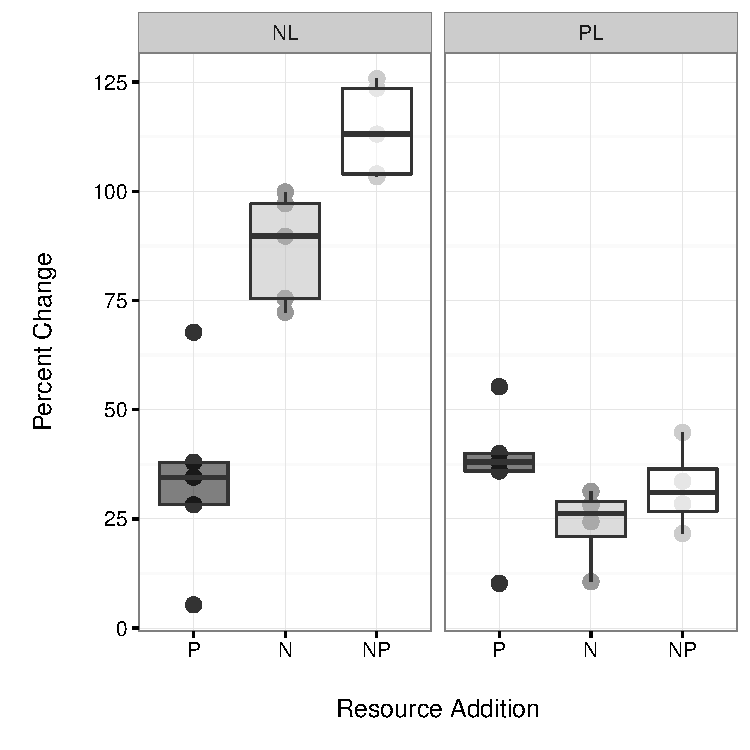
\includegraphics{analysis_ecoevostoich_files/figure-latex/perc.change-1.pdf}
\caption{Percent change in growth rate between control and nutrient
additions(N, P, or NP) cultures. NL = N-limited; PL = P-limited}
\end{figure}

\newpage

\subsubsection{Growth rate ANOVA
tables}\label{growth-rate-anova-tables-1}

\textbf{N-limited}

\begin{longtable}[]{@{}cccccc@{}}
\caption{ANOVA table for NL nutrient addition}\tabularnewline
\toprule
\begin{minipage}[b]{0.19\columnwidth}\centering\strut
~
\strut\end{minipage} &
\begin{minipage}[b]{0.06\columnwidth}\centering\strut
Df
\strut\end{minipage} &
\begin{minipage}[b]{0.10\columnwidth}\centering\strut
Sum Sq
\strut\end{minipage} &
\begin{minipage}[b]{0.12\columnwidth}\centering\strut
Mean Sq
\strut\end{minipage} &
\begin{minipage}[b]{0.12\columnwidth}\centering\strut
F value
\strut\end{minipage} &
\begin{minipage}[b]{0.12\columnwidth}\centering\strut
Pr(\textgreater{}F)
\strut\end{minipage}\tabularnewline
\midrule
\endfirsthead
\toprule
\begin{minipage}[b]{0.19\columnwidth}\centering\strut
~
\strut\end{minipage} &
\begin{minipage}[b]{0.06\columnwidth}\centering\strut
Df
\strut\end{minipage} &
\begin{minipage}[b]{0.10\columnwidth}\centering\strut
Sum Sq
\strut\end{minipage} &
\begin{minipage}[b]{0.12\columnwidth}\centering\strut
Mean Sq
\strut\end{minipage} &
\begin{minipage}[b]{0.12\columnwidth}\centering\strut
F value
\strut\end{minipage} &
\begin{minipage}[b]{0.12\columnwidth}\centering\strut
Pr(\textgreater{}F)
\strut\end{minipage}\tabularnewline
\midrule
\endhead
\begin{minipage}[t]{0.19\columnwidth}\centering\strut
\textbf{med.add}
\strut\end{minipage} &
\begin{minipage}[t]{0.06\columnwidth}\centering\strut
2
\strut\end{minipage} &
\begin{minipage}[t]{0.10\columnwidth}\centering\strut
16206
\strut\end{minipage} &
\begin{minipage}[t]{0.12\columnwidth}\centering\strut
8103
\strut\end{minipage} &
\begin{minipage}[t]{0.12\columnwidth}\centering\strut
31.59
\strut\end{minipage} &
\begin{minipage}[t]{0.12\columnwidth}\centering\strut
1.653e-05
\strut\end{minipage}\tabularnewline
\begin{minipage}[t]{0.19\columnwidth}\centering\strut
\textbf{Residuals}
\strut\end{minipage} &
\begin{minipage}[t]{0.06\columnwidth}\centering\strut
12
\strut\end{minipage} &
\begin{minipage}[t]{0.10\columnwidth}\centering\strut
3078
\strut\end{minipage} &
\begin{minipage}[t]{0.12\columnwidth}\centering\strut
256.5
\strut\end{minipage} &
\begin{minipage}[t]{0.12\columnwidth}\centering\strut
NA
\strut\end{minipage} &
\begin{minipage}[t]{0.12\columnwidth}\centering\strut
NA
\strut\end{minipage}\tabularnewline
\bottomrule
\end{longtable}

\begin{longtable}[]{@{}ccccc@{}}
\caption{Posthoc comparisons using Tukey HSD}\tabularnewline
\toprule
\begin{minipage}[b]{0.13\columnwidth}\centering\strut
~
\strut\end{minipage} &
\begin{minipage}[b]{0.13\columnwidth}\centering\strut
diff
\strut\end{minipage} &
\begin{minipage}[b]{0.14\columnwidth}\centering\strut
lwr
\strut\end{minipage} &
\begin{minipage}[b]{0.13\columnwidth}\centering\strut
upr
\strut\end{minipage} &
\begin{minipage}[b]{0.16\columnwidth}\centering\strut
p adj
\strut\end{minipage}\tabularnewline
\midrule
\endfirsthead
\toprule
\begin{minipage}[b]{0.13\columnwidth}\centering\strut
~
\strut\end{minipage} &
\begin{minipage}[b]{0.13\columnwidth}\centering\strut
diff
\strut\end{minipage} &
\begin{minipage}[b]{0.14\columnwidth}\centering\strut
lwr
\strut\end{minipage} &
\begin{minipage}[b]{0.13\columnwidth}\centering\strut
upr
\strut\end{minipage} &
\begin{minipage}[b]{0.16\columnwidth}\centering\strut
p adj
\strut\end{minipage}\tabularnewline
\midrule
\endhead
\begin{minipage}[t]{0.13\columnwidth}\centering\strut
\textbf{NP-N}
\strut\end{minipage} &
\begin{minipage}[t]{0.13\columnwidth}\centering\strut
\textbf{27.06}
\strut\end{minipage} &
\begin{minipage}[t]{0.14\columnwidth}\centering\strut
\textbf{0.03951}
\strut\end{minipage} &
\begin{minipage}[t]{0.13\columnwidth}\centering\strut
\textbf{54.08}
\strut\end{minipage} &
\begin{minipage}[t]{0.16\columnwidth}\centering\strut
\textbf{0.04966}
\strut\end{minipage}\tabularnewline
\begin{minipage}[t]{0.13\columnwidth}\centering\strut
\textbf{P-N}
\strut\end{minipage} &
\begin{minipage}[t]{0.13\columnwidth}\centering\strut
\textbf{-52.14}
\strut\end{minipage} &
\begin{minipage}[t]{0.14\columnwidth}\centering\strut
\textbf{-79.16}
\strut\end{minipage} &
\begin{minipage}[t]{0.13\columnwidth}\centering\strut
\textbf{-25.12}
\strut\end{minipage} &
\begin{minipage}[t]{0.16\columnwidth}\centering\strut
\textbf{0.0006541}
\strut\end{minipage}\tabularnewline
\begin{minipage}[t]{0.13\columnwidth}\centering\strut
\textbf{P-NP}
\strut\end{minipage} &
\begin{minipage}[t]{0.13\columnwidth}\centering\strut
\textbf{-79.2}
\strut\end{minipage} &
\begin{minipage}[t]{0.14\columnwidth}\centering\strut
\textbf{-106.2}
\strut\end{minipage} &
\begin{minipage}[t]{0.13\columnwidth}\centering\strut
\textbf{-52.18}
\strut\end{minipage} &
\begin{minipage}[t]{0.16\columnwidth}\centering\strut
\textbf{1.316e-05}
\strut\end{minipage}\tabularnewline
\bottomrule
\end{longtable}

\textbf{P-limited}

\begin{longtable}[]{@{}cccccc@{}}
\caption{ANOVA table for PL nutrient addition}\tabularnewline
\toprule
\begin{minipage}[b]{0.19\columnwidth}\centering\strut
~
\strut\end{minipage} &
\begin{minipage}[b]{0.06\columnwidth}\centering\strut
Df
\strut\end{minipage} &
\begin{minipage}[b]{0.10\columnwidth}\centering\strut
Sum Sq
\strut\end{minipage} &
\begin{minipage}[b]{0.12\columnwidth}\centering\strut
Mean Sq
\strut\end{minipage} &
\begin{minipage}[b]{0.12\columnwidth}\centering\strut
F value
\strut\end{minipage} &
\begin{minipage}[b]{0.12\columnwidth}\centering\strut
Pr(\textgreater{}F)
\strut\end{minipage}\tabularnewline
\midrule
\endfirsthead
\toprule
\begin{minipage}[b]{0.19\columnwidth}\centering\strut
~
\strut\end{minipage} &
\begin{minipage}[b]{0.06\columnwidth}\centering\strut
Df
\strut\end{minipage} &
\begin{minipage}[b]{0.10\columnwidth}\centering\strut
Sum Sq
\strut\end{minipage} &
\begin{minipage}[b]{0.12\columnwidth}\centering\strut
Mean Sq
\strut\end{minipage} &
\begin{minipage}[b]{0.12\columnwidth}\centering\strut
F value
\strut\end{minipage} &
\begin{minipage}[b]{0.12\columnwidth}\centering\strut
Pr(\textgreater{}F)
\strut\end{minipage}\tabularnewline
\midrule
\endhead
\begin{minipage}[t]{0.19\columnwidth}\centering\strut
\textbf{med.add}
\strut\end{minipage} &
\begin{minipage}[t]{0.06\columnwidth}\centering\strut
2
\strut\end{minipage} &
\begin{minipage}[t]{0.10\columnwidth}\centering\strut
343.4
\strut\end{minipage} &
\begin{minipage}[t]{0.12\columnwidth}\centering\strut
171.7
\strut\end{minipage} &
\begin{minipage}[t]{0.12\columnwidth}\centering\strut
1.079
\strut\end{minipage} &
\begin{minipage}[t]{0.12\columnwidth}\centering\strut
0.3765
\strut\end{minipage}\tabularnewline
\begin{minipage}[t]{0.19\columnwidth}\centering\strut
\textbf{Residuals}
\strut\end{minipage} &
\begin{minipage}[t]{0.06\columnwidth}\centering\strut
10
\strut\end{minipage} &
\begin{minipage}[t]{0.10\columnwidth}\centering\strut
1592
\strut\end{minipage} &
\begin{minipage}[t]{0.12\columnwidth}\centering\strut
159.2
\strut\end{minipage} &
\begin{minipage}[t]{0.12\columnwidth}\centering\strut
NA
\strut\end{minipage} &
\begin{minipage}[t]{0.12\columnwidth}\centering\strut
NA
\strut\end{minipage}\tabularnewline
\bottomrule
\end{longtable}

\begin{longtable}[]{@{}ccccc@{}}
\caption{Posthoc comparisons using Tukey HSD}\tabularnewline
\toprule
\begin{minipage}[b]{0.13\columnwidth}\centering\strut
~
\strut\end{minipage} &
\begin{minipage}[b]{0.08\columnwidth}\centering\strut
diff
\strut\end{minipage} &
\begin{minipage}[b]{0.08\columnwidth}\centering\strut
lwr
\strut\end{minipage} &
\begin{minipage}[b]{0.07\columnwidth}\centering\strut
upr
\strut\end{minipage} &
\begin{minipage}[b]{0.08\columnwidth}\centering\strut
p adj
\strut\end{minipage}\tabularnewline
\midrule
\endfirsthead
\toprule
\begin{minipage}[b]{0.13\columnwidth}\centering\strut
~
\strut\end{minipage} &
\begin{minipage}[b]{0.08\columnwidth}\centering\strut
diff
\strut\end{minipage} &
\begin{minipage}[b]{0.08\columnwidth}\centering\strut
lwr
\strut\end{minipage} &
\begin{minipage}[b]{0.07\columnwidth}\centering\strut
upr
\strut\end{minipage} &
\begin{minipage}[b]{0.08\columnwidth}\centering\strut
p adj
\strut\end{minipage}\tabularnewline
\midrule
\endhead
\begin{minipage}[t]{0.13\columnwidth}\centering\strut
\textbf{NP-N}
\strut\end{minipage} &
\begin{minipage}[t]{0.08\columnwidth}\centering\strut
8.522
\strut\end{minipage} &
\begin{minipage}[t]{0.08\columnwidth}\centering\strut
-15.93
\strut\end{minipage} &
\begin{minipage}[t]{0.07\columnwidth}\centering\strut
32.98
\strut\end{minipage} &
\begin{minipage}[t]{0.08\columnwidth}\centering\strut
0.6197
\strut\end{minipage}\tabularnewline
\begin{minipage}[t]{0.13\columnwidth}\centering\strut
\textbf{P-N}
\strut\end{minipage} &
\begin{minipage}[t]{0.08\columnwidth}\centering\strut
12.29
\strut\end{minipage} &
\begin{minipage}[t]{0.08\columnwidth}\centering\strut
-10.91
\strut\end{minipage} &
\begin{minipage}[t]{0.07\columnwidth}\centering\strut
35.49
\strut\end{minipage} &
\begin{minipage}[t]{0.08\columnwidth}\centering\strut
0.3532
\strut\end{minipage}\tabularnewline
\begin{minipage}[t]{0.13\columnwidth}\centering\strut
\textbf{P-NP}
\strut\end{minipage} &
\begin{minipage}[t]{0.08\columnwidth}\centering\strut
3.764
\strut\end{minipage} &
\begin{minipage}[t]{0.08\columnwidth}\centering\strut
-19.44
\strut\end{minipage} &
\begin{minipage}[t]{0.07\columnwidth}\centering\strut
26.96
\strut\end{minipage} &
\begin{minipage}[t]{0.08\columnwidth}\centering\strut
0.8978
\strut\end{minipage}\tabularnewline
\bottomrule
\end{longtable}

\newpage

\section{Population Dynamics: Does nutrient stoichiometry affect
temporal
dynamics?}\label{population-dynamics-does-nutrient-stoichiometry-affect-temporal-dynamics}

\textbf{Overview}: In this experiment, whole samples were collected from
each chemostat system three times per week for \textasciitilde{}5
months. Each sample was processed, stained, and counted using
epi-fluorescence on a Zeiss microscope and quantified using Axiovision
software. Statistics for these data include repeated measures anova
(RMANOVA), stability (1/CV), and cross-correlation analyses on whitened
data.

\subsection{Summary of Major Results}\label{summary-of-major-results-1}

\begin{enumerate}
\def\labelenumi{\arabic{enumi}.}
\tightlist
\item
  Stoichiometry significantly affected \emph{Synechococcus} and phage
  densities. RMANOVA
\item
  Altered mean and stability of the populations
\item
  Modified the temporal coherence, or synchrony, of the
  \emph{Synechococcus}-phage dynamics, suggesting ecological
  ramifications of stoichiometry.
\end{enumerate}

\newpage

\subsection{Chemostat-level
comparisons}\label{chemostat-level-comparisons}

\subsubsection{Population dynamics}\label{population-dynamics}

\begin{figure}[htbp]
\centering
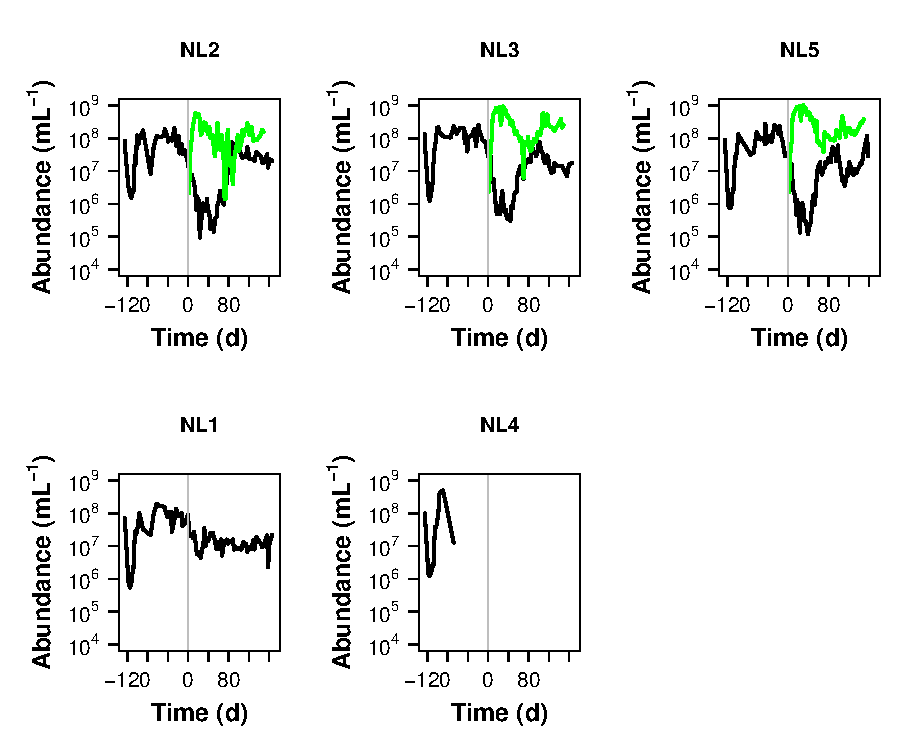
\includegraphics{analysis_ecoevostoich_files/figure-latex/unnamed-chunk-2-1.pdf}
\caption{N-Limited Chemostats}
\end{figure}

\newpage

\begin{figure}[htbp]
\centering
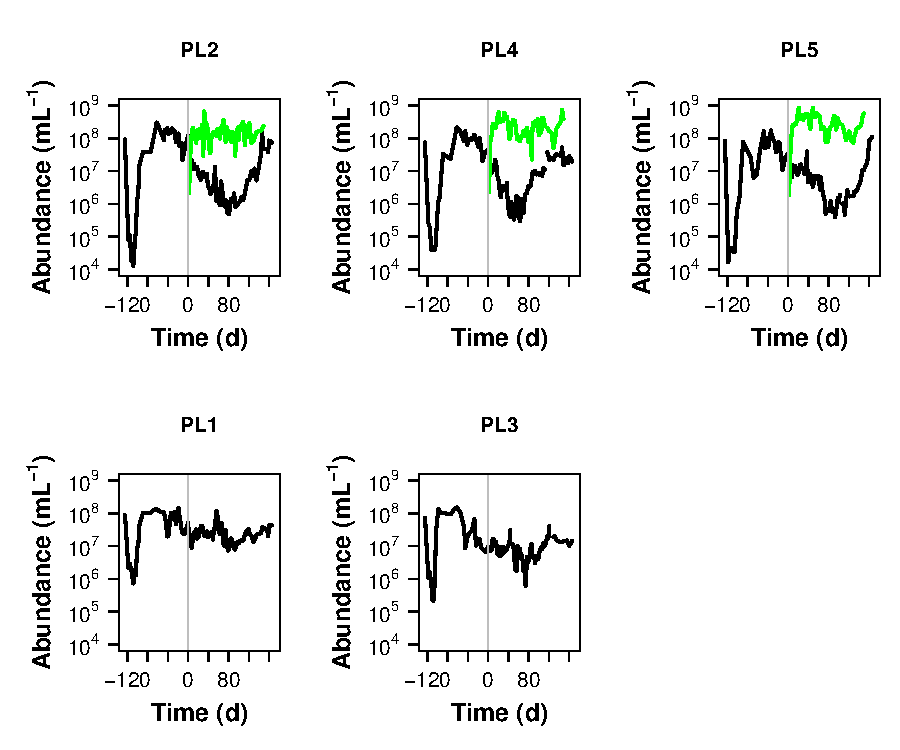
\includegraphics{analysis_ecoevostoich_files/figure-latex/unnamed-chunk-3-1.pdf}
\caption{P-Limited Chemostats}
\end{figure}

\newpage

\subsubsection{Phage to bacteria ratio}\label{phage-to-bacteria-ratio}

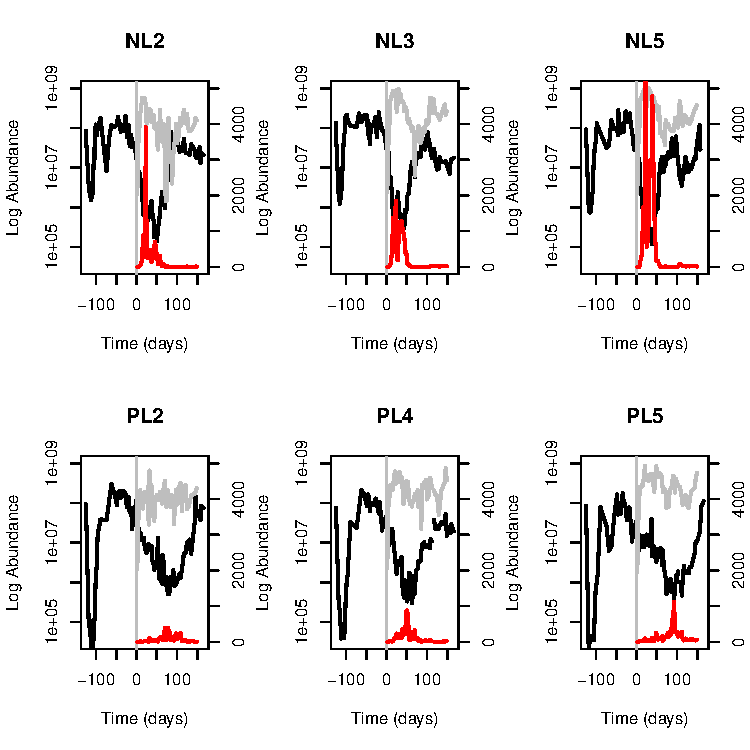
\includegraphics{analysis_ecoevostoich_files/figure-latex/unnamed-chunk-4-1.pdf}
\newpage

\subsection{Treatment-level
comparisons}\label{treatment-level-comparisons}

\subsubsection{Controls}\label{controls}

\begin{figure}[htbp]
\centering
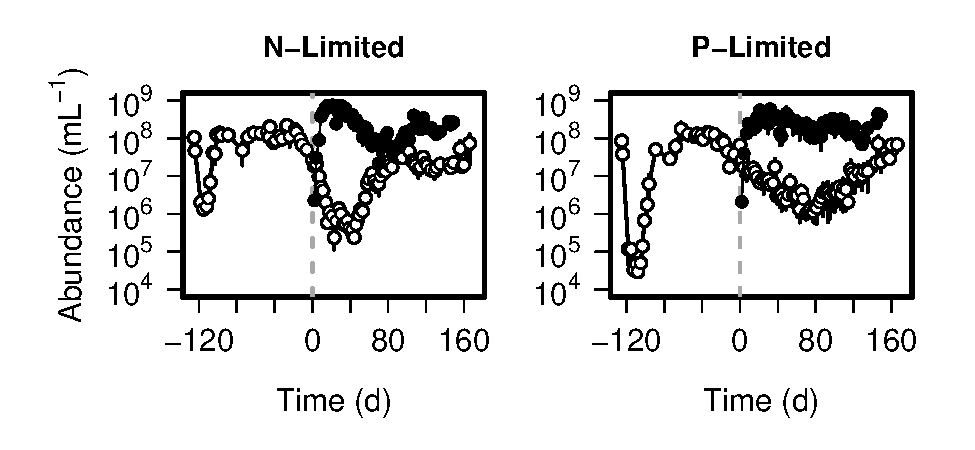
\includegraphics{analysis_ecoevostoich_files/figure-latex/unnamed-chunk-6-1.pdf}
\caption{Control Chemostats}
\end{figure}

\subsubsection{Treatment (i.e.~Exposed) population
abundances}\label{treatment-i.e.exposed-population-abundances}

\begin{figure}[htbp]
\centering
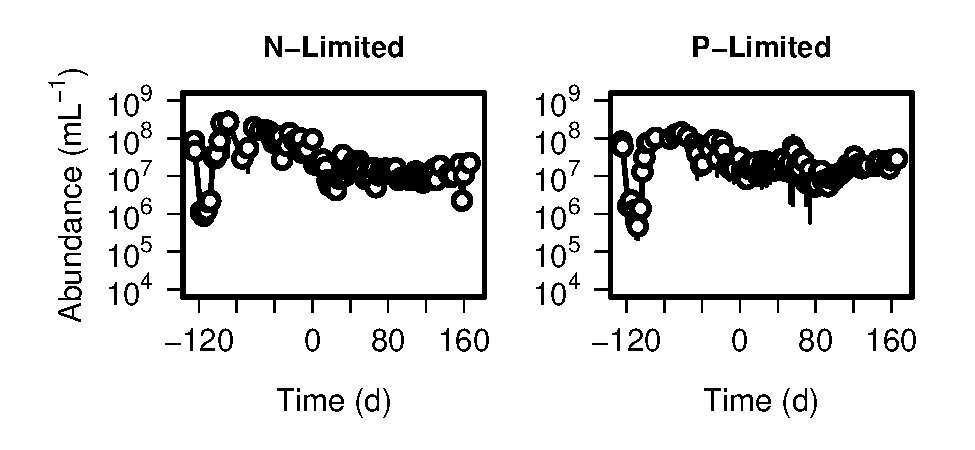
\includegraphics{analysis_ecoevostoich_files/figure-latex/unnamed-chunk-7-1.pdf}
\caption{Treatment Chemostats}
\end{figure}

\textbf{RMANOVA for control cyanobacteria}

\textbf{RMANOVA for control vs exposed cyanobacteria densities}

\newpage

\subsubsection{Temporal autocorrelation}\label{temporal-autocorrelation}

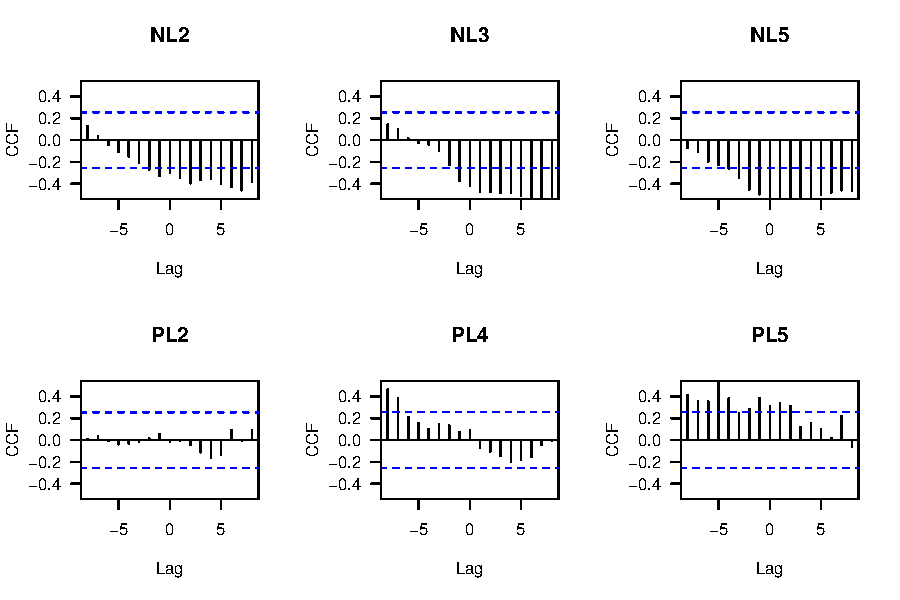
\includegraphics{analysis_ecoevostoich_files/figure-latex/unnamed-chunk-11-1.pdf}
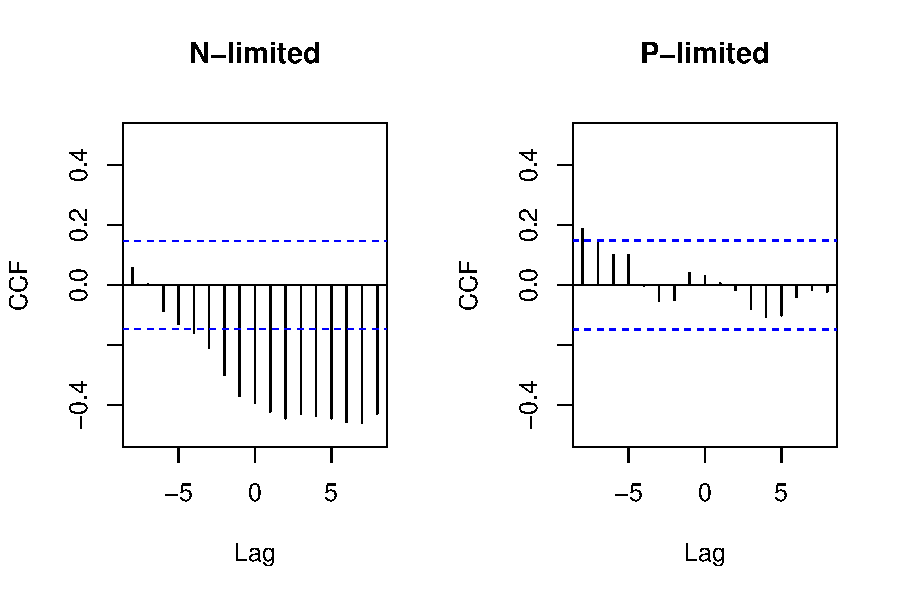
\includegraphics{analysis_ecoevostoich_files/figure-latex/unnamed-chunk-11-2.pdf}

\newpage

\subsection{Statistical analyses}\label{statistical-analyses}

\emph{NOTE}:Cross-correlation analyses and RMANOVA were also completed
in SAS

\subsubsection{Heteroskedaskicity (i.e skewness) with treatment data
only}\label{heteroskedaskicity-i.e-skewness-with-treatment-data-only}

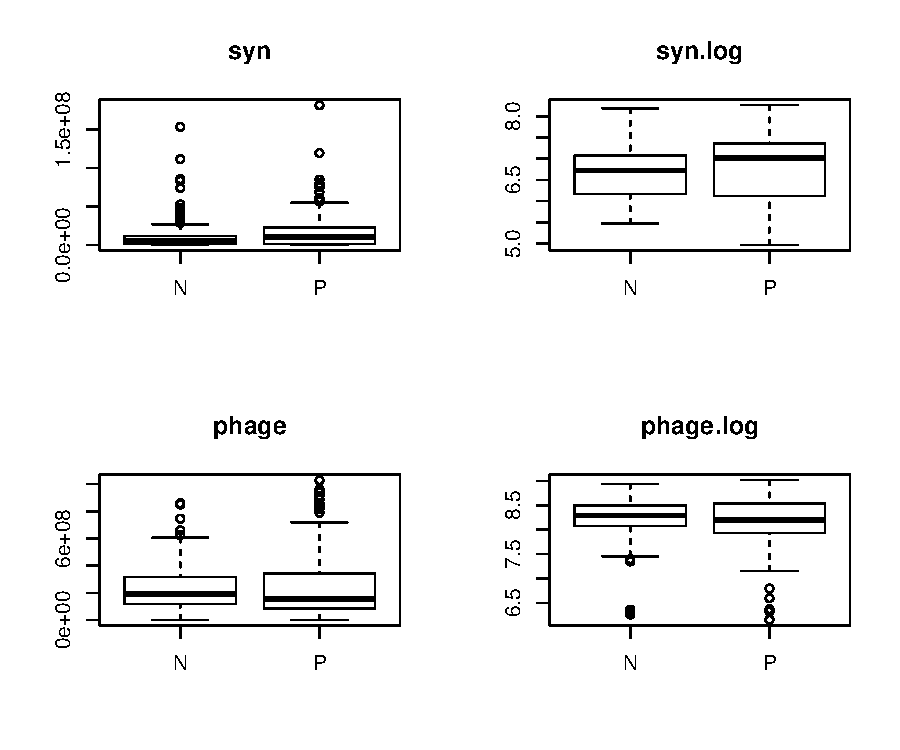
\includegraphics{analysis_ecoevostoich_files/figure-latex/unnamed-chunk-12-1.pdf}

\newpage

\subsubsection{Reapeated Measures ANOVA
(RMANOVA)}\label{reapeated-measures-anova-rmanova}

\begin{longtable}[]{@{}ccccc@{}}
\toprule
\begin{minipage}[b]{0.21\columnwidth}\centering\strut
~
\strut\end{minipage} &
\begin{minipage}[b]{0.10\columnwidth}\centering\strut
numDF
\strut\end{minipage} &
\begin{minipage}[b]{0.10\columnwidth}\centering\strut
denDF
\strut\end{minipage} &
\begin{minipage}[b]{0.12\columnwidth}\centering\strut
F-value
\strut\end{minipage} &
\begin{minipage}[b]{0.12\columnwidth}\centering\strut
p-value
\strut\end{minipage}\tabularnewline
\midrule
\endhead
\begin{minipage}[t]{0.21\columnwidth}\centering\strut
\textbf{(Intercept)}
\strut\end{minipage} &
\begin{minipage}[t]{0.10\columnwidth}\centering\strut
1
\strut\end{minipage} &
\begin{minipage}[t]{0.10\columnwidth}\centering\strut
230
\strut\end{minipage} &
\begin{minipage}[t]{0.12\columnwidth}\centering\strut
14010
\strut\end{minipage} &
\begin{minipage}[t]{0.12\columnwidth}\centering\strut
0
\strut\end{minipage}\tabularnewline
\begin{minipage}[t]{0.21\columnwidth}\centering\strut
\textbf{lim}
\strut\end{minipage} &
\begin{minipage}[t]{0.10\columnwidth}\centering\strut
1
\strut\end{minipage} &
\begin{minipage}[t]{0.10\columnwidth}\centering\strut
4
\strut\end{minipage} &
\begin{minipage}[t]{0.12\columnwidth}\centering\strut
0.3592
\strut\end{minipage} &
\begin{minipage}[t]{0.12\columnwidth}\centering\strut
0.5812
\strut\end{minipage}\tabularnewline
\begin{minipage}[t]{0.21\columnwidth}\centering\strut
\textbf{day.fac}
\strut\end{minipage} &
\begin{minipage}[t]{0.10\columnwidth}\centering\strut
58
\strut\end{minipage} &
\begin{minipage}[t]{0.10\columnwidth}\centering\strut
230
\strut\end{minipage} &
\begin{minipage}[t]{0.12\columnwidth}\centering\strut
10.22
\strut\end{minipage} &
\begin{minipage}[t]{0.12\columnwidth}\centering\strut
0
\strut\end{minipage}\tabularnewline
\begin{minipage}[t]{0.21\columnwidth}\centering\strut
\textbf{lim:day.fac}
\strut\end{minipage} &
\begin{minipage}[t]{0.10\columnwidth}\centering\strut
58
\strut\end{minipage} &
\begin{minipage}[t]{0.10\columnwidth}\centering\strut
230
\strut\end{minipage} &
\begin{minipage}[t]{0.12\columnwidth}\centering\strut
2.588
\strut\end{minipage} &
\begin{minipage}[t]{0.12\columnwidth}\centering\strut
2.771e-07
\strut\end{minipage}\tabularnewline
\bottomrule
\end{longtable}

\begin{verbatim}
##             numDF denDF  F-value p-value
## (Intercept)     1   245 987.2110  <.0001
## lim             1     4   0.1869  0.6878
## day.fac        62   245   3.3834  <.0001
## lim:day.fac    62   245   2.4368  <.0001
\end{verbatim}

\begin{longtable}[]{@{}ccccc@{}}
\toprule
\begin{minipage}[b]{0.21\columnwidth}\centering\strut
~
\strut\end{minipage} &
\begin{minipage}[b]{0.10\columnwidth}\centering\strut
numDF
\strut\end{minipage} &
\begin{minipage}[b]{0.10\columnwidth}\centering\strut
denDF
\strut\end{minipage} &
\begin{minipage}[b]{0.12\columnwidth}\centering\strut
F-value
\strut\end{minipage} &
\begin{minipage}[b]{0.12\columnwidth}\centering\strut
p-value
\strut\end{minipage}\tabularnewline
\midrule
\endhead
\begin{minipage}[t]{0.21\columnwidth}\centering\strut
\textbf{(Intercept)}
\strut\end{minipage} &
\begin{minipage}[t]{0.10\columnwidth}\centering\strut
1
\strut\end{minipage} &
\begin{minipage}[t]{0.10\columnwidth}\centering\strut
245
\strut\end{minipage} &
\begin{minipage}[t]{0.12\columnwidth}\centering\strut
12432
\strut\end{minipage} &
\begin{minipage}[t]{0.12\columnwidth}\centering\strut
0
\strut\end{minipage}\tabularnewline
\begin{minipage}[t]{0.21\columnwidth}\centering\strut
\textbf{lim}
\strut\end{minipage} &
\begin{minipage}[t]{0.10\columnwidth}\centering\strut
1
\strut\end{minipage} &
\begin{minipage}[t]{0.10\columnwidth}\centering\strut
4
\strut\end{minipage} &
\begin{minipage}[t]{0.12\columnwidth}\centering\strut
0.5225
\strut\end{minipage} &
\begin{minipage}[t]{0.12\columnwidth}\centering\strut
0.5098
\strut\end{minipage}\tabularnewline
\begin{minipage}[t]{0.21\columnwidth}\centering\strut
\textbf{day.fac}
\strut\end{minipage} &
\begin{minipage}[t]{0.10\columnwidth}\centering\strut
62
\strut\end{minipage} &
\begin{minipage}[t]{0.10\columnwidth}\centering\strut
245
\strut\end{minipage} &
\begin{minipage}[t]{0.12\columnwidth}\centering\strut
3.354
\strut\end{minipage} &
\begin{minipage}[t]{0.12\columnwidth}\centering\strut
1.14e-11
\strut\end{minipage}\tabularnewline
\begin{minipage}[t]{0.21\columnwidth}\centering\strut
\textbf{lim:day.fac}
\strut\end{minipage} &
\begin{minipage}[t]{0.10\columnwidth}\centering\strut
62
\strut\end{minipage} &
\begin{minipage}[t]{0.10\columnwidth}\centering\strut
245
\strut\end{minipage} &
\begin{minipage}[t]{0.12\columnwidth}\centering\strut
2.437
\strut\end{minipage} &
\begin{minipage}[t]{0.12\columnwidth}\centering\strut
6.993e-07
\strut\end{minipage}\tabularnewline
\bottomrule
\end{longtable}

\newpage

\subsubsection{Despcriptive statistics}\label{despcriptive-statistics}

\begin{longtable}[]{@{}cccccc@{}}
\toprule
\begin{minipage}[b]{0.07\columnwidth}\centering\strut
lim
\strut\end{minipage} &
\begin{minipage}[b]{0.07\columnwidth}\centering\strut
cID
\strut\end{minipage} &
\begin{minipage}[b]{0.12\columnwidth}\centering\strut
microbe
\strut\end{minipage} &
\begin{minipage}[b]{0.12\columnwidth}\centering\strut
mean
\strut\end{minipage} &
\begin{minipage}[b]{0.12\columnwidth}\centering\strut
var
\strut\end{minipage} &
\begin{minipage}[b]{0.12\columnwidth}\centering\strut
sem
\strut\end{minipage}\tabularnewline
\midrule
\endhead
\begin{minipage}[t]{0.07\columnwidth}\centering\strut
N
\strut\end{minipage} &
\begin{minipage}[t]{0.07\columnwidth}\centering\strut
NL2
\strut\end{minipage} &
\begin{minipage}[t]{0.12\columnwidth}\centering\strut
Phage
\strut\end{minipage} &
\begin{minipage}[t]{0.12\columnwidth}\centering\strut
151575375
\strut\end{minipage} &
\begin{minipage}[t]{0.12\columnwidth}\centering\strut
1.881e+16
\strut\end{minipage} &
\begin{minipage}[t]{0.12\columnwidth}\centering\strut
79190498
\strut\end{minipage}\tabularnewline
\begin{minipage}[t]{0.07\columnwidth}\centering\strut
N
\strut\end{minipage} &
\begin{minipage}[t]{0.07\columnwidth}\centering\strut
NL3
\strut\end{minipage} &
\begin{minipage}[t]{0.12\columnwidth}\centering\strut
Phage
\strut\end{minipage} &
\begin{minipage}[t]{0.12\columnwidth}\centering\strut
292205382
\strut\end{minipage} &
\begin{minipage}[t]{0.12\columnwidth}\centering\strut
6.38e+16
\strut\end{minipage} &
\begin{minipage}[t]{0.12\columnwidth}\centering\strut
145831435
\strut\end{minipage}\tabularnewline
\begin{minipage}[t]{0.07\columnwidth}\centering\strut
N
\strut\end{minipage} &
\begin{minipage}[t]{0.07\columnwidth}\centering\strut
NL5
\strut\end{minipage} &
\begin{minipage}[t]{0.12\columnwidth}\centering\strut
Phage
\strut\end{minipage} &
\begin{minipage}[t]{0.12\columnwidth}\centering\strut
312565642
\strut\end{minipage} &
\begin{minipage}[t]{0.12\columnwidth}\centering\strut
7.765e+16
\strut\end{minipage} &
\begin{minipage}[t]{0.12\columnwidth}\centering\strut
160881119
\strut\end{minipage}\tabularnewline
\begin{minipage}[t]{0.07\columnwidth}\centering\strut
P
\strut\end{minipage} &
\begin{minipage}[t]{0.07\columnwidth}\centering\strut
PL2
\strut\end{minipage} &
\begin{minipage}[t]{0.12\columnwidth}\centering\strut
Phage
\strut\end{minipage} &
\begin{minipage}[t]{0.12\columnwidth}\centering\strut
161267374
\strut\end{minipage} &
\begin{minipage}[t]{0.12\columnwidth}\centering\strut
1.047e+16
\strut\end{minipage} &
\begin{minipage}[t]{0.12\columnwidth}\centering\strut
59073946
\strut\end{minipage}\tabularnewline
\begin{minipage}[t]{0.07\columnwidth}\centering\strut
P
\strut\end{minipage} &
\begin{minipage}[t]{0.07\columnwidth}\centering\strut
PL4
\strut\end{minipage} &
\begin{minipage}[t]{0.12\columnwidth}\centering\strut
Phage
\strut\end{minipage} &
\begin{minipage}[t]{0.12\columnwidth}\centering\strut
243403403
\strut\end{minipage} &
\begin{minipage}[t]{0.12\columnwidth}\centering\strut
2.342e+16
\strut\end{minipage} &
\begin{minipage}[t]{0.12\columnwidth}\centering\strut
88361764
\strut\end{minipage}\tabularnewline
\begin{minipage}[t]{0.07\columnwidth}\centering\strut
P
\strut\end{minipage} &
\begin{minipage}[t]{0.07\columnwidth}\centering\strut
PL5
\strut\end{minipage} &
\begin{minipage}[t]{0.12\columnwidth}\centering\strut
Phage
\strut\end{minipage} &
\begin{minipage}[t]{0.12\columnwidth}\centering\strut
312523940
\strut\end{minipage} &
\begin{minipage}[t]{0.12\columnwidth}\centering\strut
3.66e+16
\strut\end{minipage} &
\begin{minipage}[t]{0.12\columnwidth}\centering\strut
110450827
\strut\end{minipage}\tabularnewline
\begin{minipage}[t]{0.07\columnwidth}\centering\strut
N
\strut\end{minipage} &
\begin{minipage}[t]{0.07\columnwidth}\centering\strut
NL2
\strut\end{minipage} &
\begin{minipage}[t]{0.12\columnwidth}\centering\strut
Syn
\strut\end{minipage} &
\begin{minipage}[t]{0.12\columnwidth}\centering\strut
17594096
\strut\end{minipage} &
\begin{minipage}[t]{0.12\columnwidth}\centering\strut
4.371e+14
\strut\end{minipage} &
\begin{minipage}[t]{0.12\columnwidth}\centering\strut
12070003
\strut\end{minipage}\tabularnewline
\begin{minipage}[t]{0.07\columnwidth}\centering\strut
N
\strut\end{minipage} &
\begin{minipage}[t]{0.07\columnwidth}\centering\strut
NL3
\strut\end{minipage} &
\begin{minipage}[t]{0.12\columnwidth}\centering\strut
Syn
\strut\end{minipage} &
\begin{minipage}[t]{0.12\columnwidth}\centering\strut
16110168
\strut\end{minipage} &
\begin{minipage}[t]{0.12\columnwidth}\centering\strut
3.023e+14
\strut\end{minipage} &
\begin{minipage}[t]{0.12\columnwidth}\centering\strut
10039048
\strut\end{minipage}\tabularnewline
\begin{minipage}[t]{0.07\columnwidth}\centering\strut
N
\strut\end{minipage} &
\begin{minipage}[t]{0.07\columnwidth}\centering\strut
NL5
\strut\end{minipage} &
\begin{minipage}[t]{0.12\columnwidth}\centering\strut
Syn
\strut\end{minipage} &
\begin{minipage}[t]{0.12\columnwidth}\centering\strut
16985817
\strut\end{minipage} &
\begin{minipage}[t]{0.12\columnwidth}\centering\strut
8.152e+14
\strut\end{minipage} &
\begin{minipage}[t]{0.12\columnwidth}\centering\strut
16484799
\strut\end{minipage}\tabularnewline
\begin{minipage}[t]{0.07\columnwidth}\centering\strut
P
\strut\end{minipage} &
\begin{minipage}[t]{0.07\columnwidth}\centering\strut
PL2
\strut\end{minipage} &
\begin{minipage}[t]{0.12\columnwidth}\centering\strut
Syn
\strut\end{minipage} &
\begin{minipage}[t]{0.12\columnwidth}\centering\strut
12944893
\strut\end{minipage} &
\begin{minipage}[t]{0.12\columnwidth}\centering\strut
6.116e+14
\strut\end{minipage} &
\begin{minipage}[t]{0.12\columnwidth}\centering\strut
14277915
\strut\end{minipage}\tabularnewline
\begin{minipage}[t]{0.07\columnwidth}\centering\strut
P
\strut\end{minipage} &
\begin{minipage}[t]{0.07\columnwidth}\centering\strut
PL4
\strut\end{minipage} &
\begin{minipage}[t]{0.12\columnwidth}\centering\strut
Syn
\strut\end{minipage} &
\begin{minipage}[t]{0.12\columnwidth}\centering\strut
10812795
\strut\end{minipage} &
\begin{minipage}[t]{0.12\columnwidth}\centering\strut
1.329e+14
\strut\end{minipage} &
\begin{minipage}[t]{0.12\columnwidth}\centering\strut
6655700
\strut\end{minipage}\tabularnewline
\begin{minipage}[t]{0.07\columnwidth}\centering\strut
P
\strut\end{minipage} &
\begin{minipage}[t]{0.07\columnwidth}\centering\strut
PL5
\strut\end{minipage} &
\begin{minipage}[t]{0.12\columnwidth}\centering\strut
Syn
\strut\end{minipage} &
\begin{minipage}[t]{0.12\columnwidth}\centering\strut
9399556
\strut\end{minipage} &
\begin{minipage}[t]{0.12\columnwidth}\centering\strut
3.232e+14
\strut\end{minipage} &
\begin{minipage}[t]{0.12\columnwidth}\centering\strut
10380093
\strut\end{minipage}\tabularnewline
\bottomrule
\end{longtable}

\begin{longtable}[]{@{}cccccc@{}}
\toprule
\begin{minipage}[b]{0.12\columnwidth}\centering\strut
Limitation
\strut\end{minipage} &
\begin{minipage}[b]{0.11\columnwidth}\centering\strut
Treatment
\strut\end{minipage} &
\begin{minipage}[b]{0.15\columnwidth}\centering\strut
Synechococcus mean densitiy (+/- SEM)
\strut\end{minipage} &
\begin{minipage}[b]{0.16\columnwidth}\centering\strut
Synechococcus mean stability
\strut\end{minipage} &
\begin{minipage}[b]{0.16\columnwidth}\centering\strut
Phage mean density (+/- SEM)
\strut\end{minipage} &
\begin{minipage}[b]{0.11\columnwidth}\centering\strut
Phage mean stability
\strut\end{minipage}\tabularnewline
\midrule
\endhead
\begin{minipage}[t]{0.12\columnwidth}\centering\strut
N
\strut\end{minipage} &
\begin{minipage}[t]{0.11\columnwidth}\centering\strut
Control
\strut\end{minipage} &
\begin{minipage}[t]{0.15\columnwidth}\centering\strut
1.3e+07(4e+06)
\strut\end{minipage} &
\begin{minipage}[t]{0.16\columnwidth}\centering\strut
2.1
\strut\end{minipage} &
\begin{minipage}[t]{0.16\columnwidth}\centering\strut
NaN(NA)
\strut\end{minipage} &
\begin{minipage}[t]{0.11\columnwidth}\centering\strut
NA
\strut\end{minipage}\tabularnewline
\begin{minipage}[t]{0.12\columnwidth}\centering\strut
N
\strut\end{minipage} &
\begin{minipage}[t]{0.11\columnwidth}\centering\strut
Infect
\strut\end{minipage} &
\begin{minipage}[t]{0.15\columnwidth}\centering\strut
1.7e+07(1e+07)
\strut\end{minipage} &
\begin{minipage}[t]{0.16\columnwidth}\centering\strut
0.75
\strut\end{minipage} &
\begin{minipage}[t]{0.16\columnwidth}\centering\strut
2.5e+08(1.4e+08)
\strut\end{minipage} &
\begin{minipage}[t]{0.11\columnwidth}\centering\strut
1
\strut\end{minipage}\tabularnewline
\begin{minipage}[t]{0.12\columnwidth}\centering\strut
P
\strut\end{minipage} &
\begin{minipage}[t]{0.11\columnwidth}\centering\strut
Control
\strut\end{minipage} &
\begin{minipage}[t]{0.15\columnwidth}\centering\strut
1.8e+07(9e+06)
\strut\end{minipage} &
\begin{minipage}[t]{0.16\columnwidth}\centering\strut
1.1
\strut\end{minipage} &
\begin{minipage}[t]{0.16\columnwidth}\centering\strut
NaN(NA)
\strut\end{minipage} &
\begin{minipage}[t]{0.11\columnwidth}\centering\strut
NA
\strut\end{minipage}\tabularnewline
\begin{minipage}[t]{0.12\columnwidth}\centering\strut
P
\strut\end{minipage} &
\begin{minipage}[t]{0.11\columnwidth}\centering\strut
Infect
\strut\end{minipage} &
\begin{minipage}[t]{0.15\columnwidth}\centering\strut
1.1e+07(1e+07)
\strut\end{minipage} &
\begin{minipage}[t]{0.16\columnwidth}\centering\strut
0.59
\strut\end{minipage} &
\begin{minipage}[t]{0.16\columnwidth}\centering\strut
2.4e+08(9.5e+07)
\strut\end{minipage} &
\begin{minipage}[t]{0.11\columnwidth}\centering\strut
1.5
\strut\end{minipage}\tabularnewline
\bottomrule
\end{longtable}

\begin{longtable}[]{@{}cccccc@{}}
\toprule
\begin{minipage}[b]{0.12\columnwidth}\centering\strut
Chemostat
\strut\end{minipage} &
\begin{minipage}[b]{0.12\columnwidth}\centering\strut
Treatment
\strut\end{minipage} &
\begin{minipage}[b]{0.16\columnwidth}\centering\strut
Synechococcus mean densitiy (+/- SEM)
\strut\end{minipage} &
\begin{minipage}[b]{0.16\columnwidth}\centering\strut
Synechococcus mean stability
\strut\end{minipage} &
\begin{minipage}[b]{0.17\columnwidth}\centering\strut
Phage mean density (+/- SEM)
\strut\end{minipage} &
\begin{minipage}[b]{0.12\columnwidth}\centering\strut
Phage mean stability
\strut\end{minipage}\tabularnewline
\midrule
\endhead
\begin{minipage}[t]{0.12\columnwidth}\centering\strut
NL1
\strut\end{minipage} &
\begin{minipage}[t]{0.12\columnwidth}\centering\strut
Control
\strut\end{minipage} &
\begin{minipage}[t]{0.16\columnwidth}\centering\strut
1.3e+07(4e+06)
\strut\end{minipage} &
\begin{minipage}[t]{0.16\columnwidth}\centering\strut
2.1
\strut\end{minipage} &
\begin{minipage}[t]{0.17\columnwidth}\centering\strut
NaN(NA)
\strut\end{minipage} &
\begin{minipage}[t]{0.12\columnwidth}\centering\strut
NA
\strut\end{minipage}\tabularnewline
\begin{minipage}[t]{0.12\columnwidth}\centering\strut
NL2
\strut\end{minipage} &
\begin{minipage}[t]{0.12\columnwidth}\centering\strut
Infect
\strut\end{minipage} &
\begin{minipage}[t]{0.16\columnwidth}\centering\strut
1.8e+07(1e+07)
\strut\end{minipage} &
\begin{minipage}[t]{0.16\columnwidth}\centering\strut
0.84
\strut\end{minipage} &
\begin{minipage}[t]{0.17\columnwidth}\centering\strut
1.5e+08(7.9e+07)
\strut\end{minipage} &
\begin{minipage}[t]{0.12\columnwidth}\centering\strut
1.1
\strut\end{minipage}\tabularnewline
\begin{minipage}[t]{0.12\columnwidth}\centering\strut
NL3
\strut\end{minipage} &
\begin{minipage}[t]{0.12\columnwidth}\centering\strut
Infect
\strut\end{minipage} &
\begin{minipage}[t]{0.16\columnwidth}\centering\strut
1.6e+07(1e+07)
\strut\end{minipage} &
\begin{minipage}[t]{0.16\columnwidth}\centering\strut
0.93
\strut\end{minipage} &
\begin{minipage}[t]{0.17\columnwidth}\centering\strut
2.9e+08(1.5e+08)
\strut\end{minipage} &
\begin{minipage}[t]{0.12\columnwidth}\centering\strut
1.2
\strut\end{minipage}\tabularnewline
\begin{minipage}[t]{0.12\columnwidth}\centering\strut
NL5
\strut\end{minipage} &
\begin{minipage}[t]{0.12\columnwidth}\centering\strut
Infect
\strut\end{minipage} &
\begin{minipage}[t]{0.16\columnwidth}\centering\strut
1.7e+07(2e+07)
\strut\end{minipage} &
\begin{minipage}[t]{0.16\columnwidth}\centering\strut
0.59
\strut\end{minipage} &
\begin{minipage}[t]{0.17\columnwidth}\centering\strut
3.1e+08(1.6e+08)
\strut\end{minipage} &
\begin{minipage}[t]{0.12\columnwidth}\centering\strut
1.1
\strut\end{minipage}\tabularnewline
\begin{minipage}[t]{0.12\columnwidth}\centering\strut
PL1
\strut\end{minipage} &
\begin{minipage}[t]{0.12\columnwidth}\centering\strut
Control
\strut\end{minipage} &
\begin{minipage}[t]{0.16\columnwidth}\centering\strut
2.5e+07(1e+07)
\strut\end{minipage} &
\begin{minipage}[t]{0.16\columnwidth}\centering\strut
1.4
\strut\end{minipage} &
\begin{minipage}[t]{0.17\columnwidth}\centering\strut
NaN(NA)
\strut\end{minipage} &
\begin{minipage}[t]{0.12\columnwidth}\centering\strut
NA
\strut\end{minipage}\tabularnewline
\begin{minipage}[t]{0.12\columnwidth}\centering\strut
PL2
\strut\end{minipage} &
\begin{minipage}[t]{0.12\columnwidth}\centering\strut
Infect
\strut\end{minipage} &
\begin{minipage}[t]{0.16\columnwidth}\centering\strut
1.3e+07(1e+07)
\strut\end{minipage} &
\begin{minipage}[t]{0.16\columnwidth}\centering\strut
0.52
\strut\end{minipage} &
\begin{minipage}[t]{0.17\columnwidth}\centering\strut
1.6e+08(5.9e+07)
\strut\end{minipage} &
\begin{minipage}[t]{0.12\columnwidth}\centering\strut
1.6
\strut\end{minipage}\tabularnewline
\begin{minipage}[t]{0.12\columnwidth}\centering\strut
PL3
\strut\end{minipage} &
\begin{minipage}[t]{0.12\columnwidth}\centering\strut
Control
\strut\end{minipage} &
\begin{minipage}[t]{0.16\columnwidth}\centering\strut
9864044(4e+06)
\strut\end{minipage} &
\begin{minipage}[t]{0.16\columnwidth}\centering\strut
1.4
\strut\end{minipage} &
\begin{minipage}[t]{0.17\columnwidth}\centering\strut
NaN(NA)
\strut\end{minipage} &
\begin{minipage}[t]{0.12\columnwidth}\centering\strut
NA
\strut\end{minipage}\tabularnewline
\begin{minipage}[t]{0.12\columnwidth}\centering\strut
PL4
\strut\end{minipage} &
\begin{minipage}[t]{0.12\columnwidth}\centering\strut
Infect
\strut\end{minipage} &
\begin{minipage}[t]{0.16\columnwidth}\centering\strut
1.1e+07(7e+06)
\strut\end{minipage} &
\begin{minipage}[t]{0.16\columnwidth}\centering\strut
0.94
\strut\end{minipage} &
\begin{minipage}[t]{0.17\columnwidth}\centering\strut
2.4e+08(8.8e+07)
\strut\end{minipage} &
\begin{minipage}[t]{0.12\columnwidth}\centering\strut
1.6
\strut\end{minipage}\tabularnewline
\begin{minipage}[t]{0.12\columnwidth}\centering\strut
PL5
\strut\end{minipage} &
\begin{minipage}[t]{0.12\columnwidth}\centering\strut
Infect
\strut\end{minipage} &
\begin{minipage}[t]{0.16\columnwidth}\centering\strut
9399556(1e+07)
\strut\end{minipage} &
\begin{minipage}[t]{0.16\columnwidth}\centering\strut
0.52
\strut\end{minipage} &
\begin{minipage}[t]{0.17\columnwidth}\centering\strut
3.1e+08(1.1e+08)
\strut\end{minipage} &
\begin{minipage}[t]{0.12\columnwidth}\centering\strut
1.6
\strut\end{minipage}\tabularnewline
\bottomrule
\end{longtable}

\newpage

\subsubsection{Topographic statistics}\label{topographic-statistics}

\begin{longtable}[]{@{}cccccccc@{}}
\caption{Table continues below}\tabularnewline
\toprule
\begin{minipage}[b]{0.07\columnwidth}\centering\strut
lim
\strut\end{minipage} &
\begin{minipage}[b]{0.07\columnwidth}\centering\strut
cID
\strut\end{minipage} &
\begin{minipage}[b]{0.11\columnwidth}\centering\strut
microbe
\strut\end{minipage} &
\begin{minipage}[b]{0.11\columnwidth}\centering\strut
mean
\strut\end{minipage} &
\begin{minipage}[b]{0.11\columnwidth}\centering\strut
var
\strut\end{minipage} &
\begin{minipage}[b]{0.11\columnwidth}\centering\strut
sem
\strut\end{minipage} &
\begin{minipage}[b]{0.08\columnwidth}\centering\strut
stab
\strut\end{minipage} &
\begin{minipage}[b]{0.12\columnwidth}\centering\strut
start.abd
\strut\end{minipage}\tabularnewline
\midrule
\endfirsthead
\toprule
\begin{minipage}[b]{0.07\columnwidth}\centering\strut
lim
\strut\end{minipage} &
\begin{minipage}[b]{0.07\columnwidth}\centering\strut
cID
\strut\end{minipage} &
\begin{minipage}[b]{0.11\columnwidth}\centering\strut
microbe
\strut\end{minipage} &
\begin{minipage}[b]{0.11\columnwidth}\centering\strut
mean
\strut\end{minipage} &
\begin{minipage}[b]{0.11\columnwidth}\centering\strut
var
\strut\end{minipage} &
\begin{minipage}[b]{0.11\columnwidth}\centering\strut
sem
\strut\end{minipage} &
\begin{minipage}[b]{0.08\columnwidth}\centering\strut
stab
\strut\end{minipage} &
\begin{minipage}[b]{0.12\columnwidth}\centering\strut
start.abd
\strut\end{minipage}\tabularnewline
\midrule
\endhead
\begin{minipage}[t]{0.07\columnwidth}\centering\strut
N
\strut\end{minipage} &
\begin{minipage}[t]{0.07\columnwidth}\centering\strut
NL2
\strut\end{minipage} &
\begin{minipage}[t]{0.11\columnwidth}\centering\strut
Phage
\strut\end{minipage} &
\begin{minipage}[t]{0.11\columnwidth}\centering\strut
151575375
\strut\end{minipage} &
\begin{minipage}[t]{0.11\columnwidth}\centering\strut
1.881e+16
\strut\end{minipage} &
\begin{minipage}[t]{0.11\columnwidth}\centering\strut
79190498
\strut\end{minipage} &
\begin{minipage}[t]{0.08\columnwidth}\centering\strut
1.105
\strut\end{minipage} &
\begin{minipage}[t]{0.12\columnwidth}\centering\strut
2102121
\strut\end{minipage}\tabularnewline
\begin{minipage}[t]{0.07\columnwidth}\centering\strut
N
\strut\end{minipage} &
\begin{minipage}[t]{0.07\columnwidth}\centering\strut
NL3
\strut\end{minipage} &
\begin{minipage}[t]{0.11\columnwidth}\centering\strut
Phage
\strut\end{minipage} &
\begin{minipage}[t]{0.11\columnwidth}\centering\strut
292205382
\strut\end{minipage} &
\begin{minipage}[t]{0.11\columnwidth}\centering\strut
6.38e+16
\strut\end{minipage} &
\begin{minipage}[t]{0.11\columnwidth}\centering\strut
145831435
\strut\end{minipage} &
\begin{minipage}[t]{0.08\columnwidth}\centering\strut
1.157
\strut\end{minipage} &
\begin{minipage}[t]{0.12\columnwidth}\centering\strut
2362910
\strut\end{minipage}\tabularnewline
\begin{minipage}[t]{0.07\columnwidth}\centering\strut
N
\strut\end{minipage} &
\begin{minipage}[t]{0.07\columnwidth}\centering\strut
NL5
\strut\end{minipage} &
\begin{minipage}[t]{0.11\columnwidth}\centering\strut
Phage
\strut\end{minipage} &
\begin{minipage}[t]{0.11\columnwidth}\centering\strut
312565642
\strut\end{minipage} &
\begin{minipage}[t]{0.11\columnwidth}\centering\strut
7.765e+16
\strut\end{minipage} &
\begin{minipage}[t]{0.11\columnwidth}\centering\strut
160881119
\strut\end{minipage} &
\begin{minipage}[t]{0.08\columnwidth}\centering\strut
1.122
\strut\end{minipage} &
\begin{minipage}[t]{0.12\columnwidth}\centering\strut
2299688
\strut\end{minipage}\tabularnewline
\begin{minipage}[t]{0.07\columnwidth}\centering\strut
P
\strut\end{minipage} &
\begin{minipage}[t]{0.07\columnwidth}\centering\strut
PL2
\strut\end{minipage} &
\begin{minipage}[t]{0.11\columnwidth}\centering\strut
Phage
\strut\end{minipage} &
\begin{minipage}[t]{0.11\columnwidth}\centering\strut
161267374
\strut\end{minipage} &
\begin{minipage}[t]{0.11\columnwidth}\centering\strut
1.047e+16
\strut\end{minipage} &
\begin{minipage}[t]{0.11\columnwidth}\centering\strut
59073946
\strut\end{minipage} &
\begin{minipage}[t]{0.08\columnwidth}\centering\strut
1.576
\strut\end{minipage} &
\begin{minipage}[t]{0.12\columnwidth}\centering\strut
2102121
\strut\end{minipage}\tabularnewline
\begin{minipage}[t]{0.07\columnwidth}\centering\strut
P
\strut\end{minipage} &
\begin{minipage}[t]{0.07\columnwidth}\centering\strut
PL4
\strut\end{minipage} &
\begin{minipage}[t]{0.11\columnwidth}\centering\strut
Phage
\strut\end{minipage} &
\begin{minipage}[t]{0.11\columnwidth}\centering\strut
243403403
\strut\end{minipage} &
\begin{minipage}[t]{0.11\columnwidth}\centering\strut
2.342e+16
\strut\end{minipage} &
\begin{minipage}[t]{0.11\columnwidth}\centering\strut
88361764
\strut\end{minipage} &
\begin{minipage}[t]{0.08\columnwidth}\centering\strut
1.59
\strut\end{minipage} &
\begin{minipage}[t]{0.12\columnwidth}\centering\strut
2299688
\strut\end{minipage}\tabularnewline
\begin{minipage}[t]{0.07\columnwidth}\centering\strut
P
\strut\end{minipage} &
\begin{minipage}[t]{0.07\columnwidth}\centering\strut
PL5
\strut\end{minipage} &
\begin{minipage}[t]{0.11\columnwidth}\centering\strut
Phage
\strut\end{minipage} &
\begin{minipage}[t]{0.11\columnwidth}\centering\strut
312523940
\strut\end{minipage} &
\begin{minipage}[t]{0.11\columnwidth}\centering\strut
3.66e+16
\strut\end{minipage} &
\begin{minipage}[t]{0.11\columnwidth}\centering\strut
110450827
\strut\end{minipage} &
\begin{minipage}[t]{0.08\columnwidth}\centering\strut
1.634
\strut\end{minipage} &
\begin{minipage}[t]{0.12\columnwidth}\centering\strut
1841331
\strut\end{minipage}\tabularnewline
\begin{minipage}[t]{0.07\columnwidth}\centering\strut
N
\strut\end{minipage} &
\begin{minipage}[t]{0.07\columnwidth}\centering\strut
NL2
\strut\end{minipage} &
\begin{minipage}[t]{0.11\columnwidth}\centering\strut
Syn
\strut\end{minipage} &
\begin{minipage}[t]{0.11\columnwidth}\centering\strut
17594096
\strut\end{minipage} &
\begin{minipage}[t]{0.11\columnwidth}\centering\strut
4.371e+14
\strut\end{minipage} &
\begin{minipage}[t]{0.11\columnwidth}\centering\strut
12070003
\strut\end{minipage} &
\begin{minipage}[t]{0.08\columnwidth}\centering\strut
0.8416
\strut\end{minipage} &
\begin{minipage}[t]{0.12\columnwidth}\centering\strut
9599786
\strut\end{minipage}\tabularnewline
\begin{minipage}[t]{0.07\columnwidth}\centering\strut
N
\strut\end{minipage} &
\begin{minipage}[t]{0.07\columnwidth}\centering\strut
NL3
\strut\end{minipage} &
\begin{minipage}[t]{0.11\columnwidth}\centering\strut
Syn
\strut\end{minipage} &
\begin{minipage}[t]{0.11\columnwidth}\centering\strut
16110168
\strut\end{minipage} &
\begin{minipage}[t]{0.11\columnwidth}\centering\strut
3.023e+14
\strut\end{minipage} &
\begin{minipage}[t]{0.11\columnwidth}\centering\strut
10039048
\strut\end{minipage} &
\begin{minipage}[t]{0.08\columnwidth}\centering\strut
0.9265
\strut\end{minipage} &
\begin{minipage}[t]{0.12\columnwidth}\centering\strut
22353787
\strut\end{minipage}\tabularnewline
\begin{minipage}[t]{0.07\columnwidth}\centering\strut
N
\strut\end{minipage} &
\begin{minipage}[t]{0.07\columnwidth}\centering\strut
NL5
\strut\end{minipage} &
\begin{minipage}[t]{0.11\columnwidth}\centering\strut
Syn
\strut\end{minipage} &
\begin{minipage}[t]{0.11\columnwidth}\centering\strut
16985817
\strut\end{minipage} &
\begin{minipage}[t]{0.11\columnwidth}\centering\strut
8.152e+14
\strut\end{minipage} &
\begin{minipage}[t]{0.11\columnwidth}\centering\strut
16484799
\strut\end{minipage} &
\begin{minipage}[t]{0.08\columnwidth}\centering\strut
0.5949
\strut\end{minipage} &
\begin{minipage}[t]{0.12\columnwidth}\centering\strut
23186422
\strut\end{minipage}\tabularnewline
\begin{minipage}[t]{0.07\columnwidth}\centering\strut
P
\strut\end{minipage} &
\begin{minipage}[t]{0.07\columnwidth}\centering\strut
PL2
\strut\end{minipage} &
\begin{minipage}[t]{0.11\columnwidth}\centering\strut
Syn
\strut\end{minipage} &
\begin{minipage}[t]{0.11\columnwidth}\centering\strut
12944893
\strut\end{minipage} &
\begin{minipage}[t]{0.11\columnwidth}\centering\strut
6.116e+14
\strut\end{minipage} &
\begin{minipage}[t]{0.11\columnwidth}\centering\strut
14277915
\strut\end{minipage} &
\begin{minipage}[t]{0.08\columnwidth}\centering\strut
0.5234
\strut\end{minipage} &
\begin{minipage}[t]{0.12\columnwidth}\centering\strut
42190080
\strut\end{minipage}\tabularnewline
\begin{minipage}[t]{0.07\columnwidth}\centering\strut
P
\strut\end{minipage} &
\begin{minipage}[t]{0.07\columnwidth}\centering\strut
PL4
\strut\end{minipage} &
\begin{minipage}[t]{0.11\columnwidth}\centering\strut
Syn
\strut\end{minipage} &
\begin{minipage}[t]{0.11\columnwidth}\centering\strut
10812795
\strut\end{minipage} &
\begin{minipage}[t]{0.11\columnwidth}\centering\strut
1.329e+14
\strut\end{minipage} &
\begin{minipage}[t]{0.11\columnwidth}\centering\strut
6655700
\strut\end{minipage} &
\begin{minipage}[t]{0.08\columnwidth}\centering\strut
0.938
\strut\end{minipage} &
\begin{minipage}[t]{0.12\columnwidth}\centering\strut
31571541
\strut\end{minipage}\tabularnewline
\begin{minipage}[t]{0.07\columnwidth}\centering\strut
P
\strut\end{minipage} &
\begin{minipage}[t]{0.07\columnwidth}\centering\strut
PL5
\strut\end{minipage} &
\begin{minipage}[t]{0.11\columnwidth}\centering\strut
Syn
\strut\end{minipage} &
\begin{minipage}[t]{0.11\columnwidth}\centering\strut
9399556
\strut\end{minipage} &
\begin{minipage}[t]{0.11\columnwidth}\centering\strut
3.232e+14
\strut\end{minipage} &
\begin{minipage}[t]{0.11\columnwidth}\centering\strut
10380093
\strut\end{minipage} &
\begin{minipage}[t]{0.08\columnwidth}\centering\strut
0.5228
\strut\end{minipage} &
\begin{minipage}[t]{0.12\columnwidth}\centering\strut
9874066
\strut\end{minipage}\tabularnewline
\bottomrule
\end{longtable}

\begin{longtable}[]{@{}ccccc@{}}
\toprule
\begin{minipage}[b]{0.14\columnwidth}\centering\strut
final.abd
\strut\end{minipage} &
\begin{minipage}[b]{0.12\columnwidth}\centering\strut
min.day
\strut\end{minipage} &
\begin{minipage}[b]{0.12\columnwidth}\centering\strut
min.abd
\strut\end{minipage} &
\begin{minipage}[b]{0.12\columnwidth}\centering\strut
max.day
\strut\end{minipage} &
\begin{minipage}[b]{0.12\columnwidth}\centering\strut
max.abd
\strut\end{minipage}\tabularnewline
\midrule
\endhead
\begin{minipage}[t]{0.14\columnwidth}\centering\strut
157137459
\strut\end{minipage} &
\begin{minipage}[t]{0.12\columnwidth}\centering\strut
72
\strut\end{minipage} &
\begin{minipage}[t]{0.12\columnwidth}\centering\strut
1422488
\strut\end{minipage} &
\begin{minipage}[t]{0.12\columnwidth}\centering\strut
16
\strut\end{minipage} &
\begin{minipage}[t]{0.12\columnwidth}\centering\strut
573074216
\strut\end{minipage}\tabularnewline
\begin{minipage}[t]{0.14\columnwidth}\centering\strut
261895765
\strut\end{minipage} &
\begin{minipage}[t]{0.12\columnwidth}\centering\strut
2
\strut\end{minipage} &
\begin{minipage}[t]{0.12\columnwidth}\centering\strut
2362910
\strut\end{minipage} &
\begin{minipage}[t]{0.12\columnwidth}\centering\strut
30
\strut\end{minipage} &
\begin{minipage}[t]{0.12\columnwidth}\centering\strut
940323547
\strut\end{minipage}\tabularnewline
\begin{minipage}[t]{0.14\columnwidth}\centering\strut
378381691
\strut\end{minipage} &
\begin{minipage}[t]{0.12\columnwidth}\centering\strut
2
\strut\end{minipage} &
\begin{minipage}[t]{0.12\columnwidth}\centering\strut
2299688
\strut\end{minipage} &
\begin{minipage}[t]{0.12\columnwidth}\centering\strut
30
\strut\end{minipage} &
\begin{minipage}[t]{0.12\columnwidth}\centering\strut
1.029e+09
\strut\end{minipage}\tabularnewline
\begin{minipage}[t]{0.14\columnwidth}\centering\strut
237940680
\strut\end{minipage} &
\begin{minipage}[t]{0.12\columnwidth}\centering\strut
2
\strut\end{minipage} &
\begin{minipage}[t]{0.12\columnwidth}\centering\strut
2102121
\strut\end{minipage} &
\begin{minipage}[t]{0.12\columnwidth}\centering\strut
32
\strut\end{minipage} &
\begin{minipage}[t]{0.12\columnwidth}\centering\strut
659870095
\strut\end{minipage}\tabularnewline
\begin{minipage}[t]{0.14\columnwidth}\centering\strut
378302664
\strut\end{minipage} &
\begin{minipage}[t]{0.12\columnwidth}\centering\strut
2
\strut\end{minipage} &
\begin{minipage}[t]{0.12\columnwidth}\centering\strut
2299688
\strut\end{minipage} &
\begin{minipage}[t]{0.12\columnwidth}\centering\strut
146
\strut\end{minipage} &
\begin{minipage}[t]{0.12\columnwidth}\centering\strut
7.46e+08
\strut\end{minipage}\tabularnewline
\begin{minipage}[t]{0.14\columnwidth}\centering\strut
5.74e+08
\strut\end{minipage} &
\begin{minipage}[t]{0.12\columnwidth}\centering\strut
2
\strut\end{minipage} &
\begin{minipage}[t]{0.12\columnwidth}\centering\strut
1841331
\strut\end{minipage} &
\begin{minipage}[t]{0.12\columnwidth}\centering\strut
21
\strut\end{minipage} &
\begin{minipage}[t]{0.12\columnwidth}\centering\strut
859404750
\strut\end{minipage}\tabularnewline
\begin{minipage}[t]{0.14\columnwidth}\centering\strut
20629744
\strut\end{minipage} &
\begin{minipage}[t]{0.12\columnwidth}\centering\strut
23
\strut\end{minipage} &
\begin{minipage}[t]{0.12\columnwidth}\centering\strut
93339
\strut\end{minipage} &
\begin{minipage}[t]{0.12\columnwidth}\centering\strut
98
\strut\end{minipage} &
\begin{minipage}[t]{0.12\columnwidth}\centering\strut
84902597
\strut\end{minipage}\tabularnewline
\begin{minipage}[t]{0.14\columnwidth}\centering\strut
17710626
\strut\end{minipage} &
\begin{minipage}[t]{0.12\columnwidth}\centering\strut
44
\strut\end{minipage} &
\begin{minipage}[t]{0.12\columnwidth}\centering\strut
300299
\strut\end{minipage} &
\begin{minipage}[t]{0.12\columnwidth}\centering\strut
100
\strut\end{minipage} &
\begin{minipage}[t]{0.12\columnwidth}\centering\strut
80035767
\strut\end{minipage}\tabularnewline
\begin{minipage}[t]{0.14\columnwidth}\centering\strut
1.82e+08
\strut\end{minipage} &
\begin{minipage}[t]{0.12\columnwidth}\centering\strut
39
\strut\end{minipage} &
\begin{minipage}[t]{0.12\columnwidth}\centering\strut
117089
\strut\end{minipage} &
\begin{minipage}[t]{0.12\columnwidth}\centering\strut
166
\strut\end{minipage} &
\begin{minipage}[t]{0.12\columnwidth}\centering\strut
1.82e+08
\strut\end{minipage}\tabularnewline
\begin{minipage}[t]{0.14\columnwidth}\centering\strut
74192632
\strut\end{minipage} &
\begin{minipage}[t]{0.12\columnwidth}\centering\strut
79
\strut\end{minipage} &
\begin{minipage}[t]{0.12\columnwidth}\centering\strut
496642
\strut\end{minipage} &
\begin{minipage}[t]{0.12\columnwidth}\centering\strut
146
\strut\end{minipage} &
\begin{minipage}[t]{0.12\columnwidth}\centering\strut
153895345
\strut\end{minipage}\tabularnewline
\begin{minipage}[t]{0.14\columnwidth}\centering\strut
19439567
\strut\end{minipage} &
\begin{minipage}[t]{0.12\columnwidth}\centering\strut
63
\strut\end{minipage} &
\begin{minipage}[t]{0.12\columnwidth}\centering\strut
297912
\strut\end{minipage} &
\begin{minipage}[t]{0.12\columnwidth}\centering\strut
146
\strut\end{minipage} &
\begin{minipage}[t]{0.12\columnwidth}\centering\strut
52700866
\strut\end{minipage}\tabularnewline
\begin{minipage}[t]{0.14\columnwidth}\centering\strut
111891383
\strut\end{minipage} &
\begin{minipage}[t]{0.12\columnwidth}\centering\strut
93
\strut\end{minipage} &
\begin{minipage}[t]{0.12\columnwidth}\centering\strut
393297
\strut\end{minipage} &
\begin{minipage}[t]{0.12\columnwidth}\centering\strut
166
\strut\end{minipage} &
\begin{minipage}[t]{0.12\columnwidth}\centering\strut
111891383
\strut\end{minipage}\tabularnewline
\bottomrule
\end{longtable}

\begin{longtable}[]{@{}cccc@{}}
\toprule
\begin{minipage}[b]{0.12\columnwidth}\centering\strut
microbe
\strut\end{minipage} &
\begin{minipage}[b]{0.14\columnwidth}\centering\strut
analysis
\strut\end{minipage} &
\begin{minipage}[b]{0.06\columnwidth}\centering\strut
df
\strut\end{minipage} &
\begin{minipage}[b]{0.10\columnwidth}\centering\strut
pvalue
\strut\end{minipage}\tabularnewline
\midrule
\endhead
\begin{minipage}[t]{0.12\columnwidth}\centering\strut
syn
\strut\end{minipage} &
\begin{minipage}[t]{0.14\columnwidth}\centering\strut
mean
\strut\end{minipage} &
\begin{minipage}[t]{0.06\columnwidth}\centering\strut
2.68
\strut\end{minipage} &
\begin{minipage}[t]{0.10\columnwidth}\centering\strut
0.01793
\strut\end{minipage}\tabularnewline
\begin{minipage}[t]{0.12\columnwidth}\centering\strut
syn
\strut\end{minipage} &
\begin{minipage}[t]{0.14\columnwidth}\centering\strut
stability
\strut\end{minipage} &
\begin{minipage}[t]{0.06\columnwidth}\centering\strut
3.63
\strut\end{minipage} &
\begin{minipage}[t]{0.10\columnwidth}\centering\strut
0.5036
\strut\end{minipage}\tabularnewline
\begin{minipage}[t]{0.12\columnwidth}\centering\strut
phage
\strut\end{minipage} &
\begin{minipage}[t]{0.14\columnwidth}\centering\strut
mean
\strut\end{minipage} &
\begin{minipage}[t]{0.06\columnwidth}\centering\strut
3.92
\strut\end{minipage} &
\begin{minipage}[t]{0.10\columnwidth}\centering\strut
0.855
\strut\end{minipage}\tabularnewline
\begin{minipage}[t]{0.12\columnwidth}\centering\strut
phage
\strut\end{minipage} &
\begin{minipage}[t]{0.14\columnwidth}\centering\strut
stability
\strut\end{minipage} &
\begin{minipage}[t]{0.06\columnwidth}\centering\strut
3.94
\strut\end{minipage} &
\begin{minipage}[t]{0.10\columnwidth}\centering\strut
4e-05
\strut\end{minipage}\tabularnewline
\bottomrule
\end{longtable}

\newpage

\subsubsection{Temporal Synchrony}\label{temporal-synchrony}

\section{Infection Dynamics: Does stoichiometry alter phenotypic
(co)evolution in cyanobacteria and
phage?}\label{infection-dynamics-does-stoichiometry-alter-phenotypic-coevolution-in-cyanobacteria-and-phage}

\textbf{Overview}: To examine how nutrient stoichiometry impact
evolutionary interactions, I collected cross-infectivity data from 96
phage and \textasciitilde{}200 \emph{Synechococcus} strains. Each
challenge was recorded based on cellular growth where lysis = 1
(i.e.~infectious interaction occured) or no lysis (i.e.~no evidence of
infection; cell line is resistant). This data was incorporated into
network-based metrics.

\subsection{Summary of Major Results}\label{summary-of-major-results-2}

\begin{enumerate}
\def\labelenumi{\arabic{enumi}.}
\tightlist
\item
  \textbf{Are temporal infection dynamics affected by stoichiometry?}
\item
  \textbf{Do community infection networks change as a result of the
  environment?}
\item
  \textbf{How are the dynamics affected? Through changes in overall
  resistance/infectivity? Changes in compositional resistance?}
\end{enumerate}

\newpage

\subsection{Degree of interaction}\label{degree-of-interaction}

\subsection{RMANOVA}\label{rmanova}

\begin{longtable}[]{@{}cccccc@{}}
\toprule
\begin{minipage}[b]{0.21\columnwidth}\centering\strut
~
\strut\end{minipage} &
\begin{minipage}[b]{0.07\columnwidth}\centering\strut
AIC
\strut\end{minipage} &
\begin{minipage}[b]{0.07\columnwidth}\centering\strut
BIC
\strut\end{minipage} &
\begin{minipage}[b]{0.10\columnwidth}\centering\strut
logLik
\strut\end{minipage} &
\begin{minipage}[b]{0.12\columnwidth}\centering\strut
L.Ratio
\strut\end{minipage} &
\begin{minipage}[b]{0.12\columnwidth}\centering\strut
p-value
\strut\end{minipage}\tabularnewline
\midrule
\endhead
\begin{minipage}[t]{0.21\columnwidth}\centering\strut
\textbf{model.ar}
\strut\end{minipage} &
\begin{minipage}[t]{0.07\columnwidth}\centering\strut
254.3
\strut\end{minipage} &
\begin{minipage}[t]{0.07\columnwidth}\centering\strut
329
\strut\end{minipage} &
\begin{minipage}[t]{0.10\columnwidth}\centering\strut
-108.2
\strut\end{minipage} &
\begin{minipage}[t]{0.12\columnwidth}\centering\strut
NA
\strut\end{minipage} &
\begin{minipage}[t]{0.12\columnwidth}\centering\strut
NA
\strut\end{minipage}\tabularnewline
\begin{minipage}[t]{0.21\columnwidth}\centering\strut
\textbf{model.arma1}
\strut\end{minipage} &
\begin{minipage}[t]{0.07\columnwidth}\centering\strut
233.7
\strut\end{minipage} &
\begin{minipage}[t]{0.07\columnwidth}\centering\strut
312.3
\strut\end{minipage} &
\begin{minipage}[t]{0.10\columnwidth}\centering\strut
-96.86
\strut\end{minipage} &
\begin{minipage}[t]{0.12\columnwidth}\centering\strut
22.59
\strut\end{minipage} &
\begin{minipage}[t]{0.12\columnwidth}\centering\strut
2.003e-06
\strut\end{minipage}\tabularnewline
\begin{minipage}[t]{0.21\columnwidth}\centering\strut
\textbf{model.arma2}
\strut\end{minipage} &
\begin{minipage}[t]{0.07\columnwidth}\centering\strut
225.7
\strut\end{minipage} &
\begin{minipage}[t]{0.07\columnwidth}\centering\strut
308.2
\strut\end{minipage} &
\begin{minipage}[t]{0.10\columnwidth}\centering\strut
-91.84
\strut\end{minipage} &
\begin{minipage}[t]{0.12\columnwidth}\centering\strut
10.05
\strut\end{minipage} &
\begin{minipage}[t]{0.12\columnwidth}\centering\strut
0.001523
\strut\end{minipage}\tabularnewline
\bottomrule
\end{longtable}

\begin{longtable}[]{@{}llll@{}}
\toprule
\begin{minipage}[b]{0.43\columnwidth}\raggedright\strut
~
\strut\end{minipage} &
\begin{minipage}[b]{0.17\columnwidth}\raggedright\strut
Std.Error
\strut\end{minipage} &
\begin{minipage}[b]{0.13\columnwidth}\raggedright\strut
t-value
\strut\end{minipage} &
\begin{minipage}[b]{0.16\columnwidth}\raggedright\strut
p-value
\strut\end{minipage}\tabularnewline
\midrule
\endhead
\begin{minipage}[t]{0.43\columnwidth}\raggedright\strut
\textbf{(Intercept)}
\strut\end{minipage} &
\begin{minipage}[t]{0.17\columnwidth}\raggedright\strut
\textbf{0.08346}
\strut\end{minipage} &
\begin{minipage}[t]{0.13\columnwidth}\raggedright\strut
\textbf{9.123}
\strut\end{minipage} &
\begin{minipage}[t]{0.16\columnwidth}\raggedright\strut
\textbf{4.674e-18}
\strut\end{minipage}\tabularnewline
\begin{minipage}[t]{0.43\columnwidth}\raggedright\strut
\textbf{trtT}
\strut\end{minipage} &
\begin{minipage}[t]{0.17\columnwidth}\raggedright\strut
\textbf{0.1136}
\strut\end{minipage} &
\begin{minipage}[t]{0.13\columnwidth}\raggedright\strut
\textbf{-2.871}
\strut\end{minipage} &
\begin{minipage}[t]{0.16\columnwidth}\raggedright\strut
\textbf{0.004325}
\strut\end{minipage}\tabularnewline
\begin{minipage}[t]{0.43\columnwidth}\raggedright\strut
\textbf{limP}
\strut\end{minipage} &
\begin{minipage}[t]{0.17\columnwidth}\raggedright\strut
\textbf{0.1155}
\strut\end{minipage} &
\begin{minipage}[t]{0.13\columnwidth}\raggedright\strut
\textbf{-3.857}
\strut\end{minipage} &
\begin{minipage}[t]{0.16\columnwidth}\raggedright\strut
\textbf{0.01819}
\strut\end{minipage}\tabularnewline
\begin{minipage}[t]{0.43\columnwidth}\raggedright\strut
\textbf{phage.time}
\strut\end{minipage} &
\begin{minipage}[t]{0.17\columnwidth}\raggedright\strut
0.0006714
\strut\end{minipage} &
\begin{minipage}[t]{0.13\columnwidth}\raggedright\strut
-1.743
\strut\end{minipage} &
\begin{minipage}[t]{0.16\columnwidth}\raggedright\strut
0.08219
\strut\end{minipage}\tabularnewline
\begin{minipage}[t]{0.43\columnwidth}\raggedright\strut
\textbf{bac.time}
\strut\end{minipage} &
\begin{minipage}[t]{0.17\columnwidth}\raggedright\strut
0.001086
\strut\end{minipage} &
\begin{minipage}[t]{0.13\columnwidth}\raggedright\strut
0.0845
\strut\end{minipage} &
\begin{minipage}[t]{0.16\columnwidth}\raggedright\strut
0.9327
\strut\end{minipage}\tabularnewline
\begin{minipage}[t]{0.43\columnwidth}\raggedright\strut
\textbf{trtT:limP}
\strut\end{minipage} &
\begin{minipage}[t]{0.17\columnwidth}\raggedright\strut
0.1588
\strut\end{minipage} &
\begin{minipage}[t]{0.13\columnwidth}\raggedright\strut
1.295
\strut\end{minipage} &
\begin{minipage}[t]{0.16\columnwidth}\raggedright\strut
0.196
\strut\end{minipage}\tabularnewline
\begin{minipage}[t]{0.43\columnwidth}\raggedright\strut
\textbf{trtT:phage.time}
\strut\end{minipage} &
\begin{minipage}[t]{0.17\columnwidth}\raggedright\strut
0.0009219
\strut\end{minipage} &
\begin{minipage}[t]{0.13\columnwidth}\raggedright\strut
0.7362
\strut\end{minipage} &
\begin{minipage}[t]{0.16\columnwidth}\raggedright\strut
0.4621
\strut\end{minipage}\tabularnewline
\begin{minipage}[t]{0.43\columnwidth}\raggedright\strut
\textbf{limP:phage.time}
\strut\end{minipage} &
\begin{minipage}[t]{0.17\columnwidth}\raggedright\strut
\textbf{0.0009172}
\strut\end{minipage} &
\begin{minipage}[t]{0.13\columnwidth}\raggedright\strut
\textbf{2.812}
\strut\end{minipage} &
\begin{minipage}[t]{0.16\columnwidth}\raggedright\strut
\textbf{0.005188}
\strut\end{minipage}\tabularnewline
\begin{minipage}[t]{0.43\columnwidth}\raggedright\strut
\textbf{trtT:bac.time}
\strut\end{minipage} &
\begin{minipage}[t]{0.17\columnwidth}\raggedright\strut
\textbf{0.001379}
\strut\end{minipage} &
\begin{minipage}[t]{0.13\columnwidth}\raggedright\strut
\textbf{-2.373}
\strut\end{minipage} &
\begin{minipage}[t]{0.16\columnwidth}\raggedright\strut
\textbf{0.01815}
\strut\end{minipage}\tabularnewline
\begin{minipage}[t]{0.43\columnwidth}\raggedright\strut
\textbf{limP:bac.time}
\strut\end{minipage} &
\begin{minipage}[t]{0.17\columnwidth}\raggedright\strut
0.001367
\strut\end{minipage} &
\begin{minipage}[t]{0.13\columnwidth}\raggedright\strut
-0.06095
\strut\end{minipage} &
\begin{minipage}[t]{0.16\columnwidth}\raggedright\strut
0.9514
\strut\end{minipage}\tabularnewline
\begin{minipage}[t]{0.43\columnwidth}\raggedright\strut
\textbf{phage.time:bac.time}
\strut\end{minipage} &
\begin{minipage}[t]{0.17\columnwidth}\raggedright\strut
9.204e-06
\strut\end{minipage} &
\begin{minipage}[t]{0.13\columnwidth}\raggedright\strut
-1.641
\strut\end{minipage} &
\begin{minipage}[t]{0.16\columnwidth}\raggedright\strut
0.1016
\strut\end{minipage}\tabularnewline
\begin{minipage}[t]{0.43\columnwidth}\raggedright\strut
\textbf{trtT:limP:phage.time}
\strut\end{minipage} &
\begin{minipage}[t]{0.17\columnwidth}\raggedright\strut
0.001273
\strut\end{minipage} &
\begin{minipage}[t]{0.13\columnwidth}\raggedright\strut
-0.6152
\strut\end{minipage} &
\begin{minipage}[t]{0.16\columnwidth}\raggedright\strut
0.5388
\strut\end{minipage}\tabularnewline
\begin{minipage}[t]{0.43\columnwidth}\raggedright\strut
\textbf{trtT:limP:bac.time}
\strut\end{minipage} &
\begin{minipage}[t]{0.17\columnwidth}\raggedright\strut
0.001816
\strut\end{minipage} &
\begin{minipage}[t]{0.13\columnwidth}\raggedright\strut
1.275
\strut\end{minipage} &
\begin{minipage}[t]{0.16\columnwidth}\raggedright\strut
0.2029
\strut\end{minipage}\tabularnewline
\begin{minipage}[t]{0.43\columnwidth}\raggedright\strut
\textbf{trtT:phage.time:bac.time}
\strut\end{minipage} &
\begin{minipage}[t]{0.17\columnwidth}\raggedright\strut
1.15e-05
\strut\end{minipage} &
\begin{minipage}[t]{0.13\columnwidth}\raggedright\strut
1.662
\strut\end{minipage} &
\begin{minipage}[t]{0.16\columnwidth}\raggedright\strut
0.09738
\strut\end{minipage}\tabularnewline
\begin{minipage}[t]{0.43\columnwidth}\raggedright\strut
\textbf{limP:phage.time:bac.time}
\strut\end{minipage} &
\begin{minipage}[t]{0.17\columnwidth}\raggedright\strut
1.145e-05
\strut\end{minipage} &
\begin{minipage}[t]{0.13\columnwidth}\raggedright\strut
0.3174
\strut\end{minipage} &
\begin{minipage}[t]{0.16\columnwidth}\raggedright\strut
0.7511
\strut\end{minipage}\tabularnewline
\begin{minipage}[t]{0.43\columnwidth}\raggedright\strut
\textbf{trtT:limP:phage.time:bac.time}
\strut\end{minipage} &
\begin{minipage}[t]{0.17\columnwidth}\raggedright\strut
1.498e-05
\strut\end{minipage} &
\begin{minipage}[t]{0.13\columnwidth}\raggedright\strut
-1.448
\strut\end{minipage} &
\begin{minipage}[t]{0.16\columnwidth}\raggedright\strut
0.1484
\strut\end{minipage}\tabularnewline
\bottomrule
\end{longtable}

\newpage

\subsection{Infection dynamics by
chemostat}\label{infection-dynamics-by-chemostat}

\newpage

\subsection{Infection dynamics by
treatment}\label{infection-dynamics-by-treatment}

\subsubsection{Network plots}\label{network-plots}

\begin{verbatim}
##       [,1] [,2] [,3] [,4] [,5] [,6] [,7] [,8] [,9] [,10] [,11] [,12] [,13]
##  [1,]    0    0    0    0    0    0    0    0    0     0     0     0     0
##  [2,]    0    0    0    0    0    0    0    0    0     0     0     0     0
##  [3,]    0    0    0    0    0    0    0    0    0     0     0     0     0
##  [4,]    0    0    0    0    0    0    0    0    0     0     0     0     0
##  [5,]    0    0    0    0    0    0    0    0    0     0     0     0     0
##  [6,]    0    0    0    0    0    0    0    0    0     0     0     0     0
##  [7,]    0    0    0    0    0    0    0    0    0     0     0     0     0
##  [8,]    0    0    0    0    0    0    0    0    0     0     0     0     0
##  [9,]    0    0    0    0    0    0    0    0    0     0     0     0     0
## [10,]    0    0    0    0    0    0    0    0    0     0     0     0     0
## [11,]    0    0    0    0    0    0    0    0    0     0     0     0     0
## [12,]    0    0    0    0    0    0    0    0    0     0     0     0     0
## [13,]    0    0    0    0    0    0    0    0    0     0     0     0     0
## [14,]    0    0    0    0    0    0    0    0    0     0     0     0     0
## [15,]    0    0    0    0    0    0    0    0    0     0     0     0     0
## [16,]    0    0    0    0    0    0    0    0    0     0     0     0     0
## [17,]    0    0    0    0    0    0    0    0    0     0     0     0     0
## [18,]    0    0    0    0    0    0    0    0    0     0     0     0     0
## [19,]    0    0    0    0    0    0    0    0    0     0     0     0     0
##       [,14] [,15] [,16] [,17] [,18] [,19]
##  [1,]     0     0     0     0     0     0
##  [2,]     0     0     0     0     0     0
##  [3,]     0     0     0     0     0     0
##  [4,]     0     0     0     0     0     0
##  [5,]     0     0     0     0     0     0
##  [6,]     0     0     0     0     0     0
##  [7,]     0     0     0     0     0     0
##  [8,]     0     0     0     0     0     0
##  [9,]     0     0     0     0     0     0
## [10,]     0     0     0     0     0     0
## [11,]     0     0     0     0     0     0
## [12,]     0     0     0     0     0     0
## [13,]     0     0     0     0     0     0
## [14,]     0     0     0     0     0     0
## [15,]     0     0     0     0     0     0
## [16,]     0     0     0     0     0     0
## [17,]     0     0     0     0     0     0
## [18,]     0     0     0     0     0     0
## [19,]     0     0     0     0     0     0
\end{verbatim}

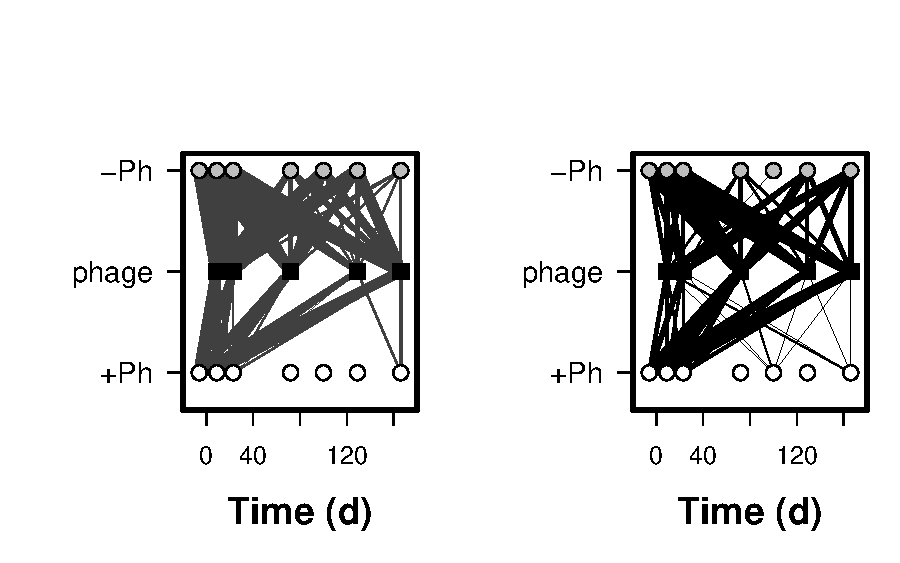
\includegraphics{analysis_ecoevostoich_files/figure-latex/coevo-pub/fig-1.pdf}

\begin{verbatim}
## null device 
##           1
\end{verbatim}

\newpage

\subsection{Community Networks}\label{community-networks}

\newpage

\subsection{BiWeb estimates for nestedness and
modularity}\label{biweb-estimates-for-nestedness-and-modularity}

\begin{longtable}[]{@{}cccc@{}}
\toprule
\begin{minipage}[b]{0.24\columnwidth}\centering\strut
~
\strut\end{minipage} &
\begin{minipage}[b]{0.23\columnwidth}\centering\strut
statistic.t
\strut\end{minipage} &
\begin{minipage}[b]{0.20\columnwidth}\centering\strut
parameter.df
\strut\end{minipage} &
\begin{minipage}[b]{0.22\columnwidth}\centering\strut
p.value
\strut\end{minipage}\tabularnewline
\midrule
\endhead
\begin{minipage}[t]{0.24\columnwidth}\centering\strut
\textbf{connectance}
\strut\end{minipage} &
\begin{minipage}[t]{0.23\columnwidth}\centering\strut
1.456400410208
\strut\end{minipage} &
\begin{minipage}[t]{0.20\columnwidth}\centering\strut
3.89610299683149
\strut\end{minipage} &
\begin{minipage}[t]{0.22\columnwidth}\centering\strut
0.220826873899216
\strut\end{minipage}\tabularnewline
\begin{minipage}[t]{0.24\columnwidth}\centering\strut
\textbf{modularity.qb}
\strut\end{minipage} &
\begin{minipage}[t]{0.23\columnwidth}\centering\strut
-3.5488938188692
\strut\end{minipage} &
\begin{minipage}[t]{0.20\columnwidth}\centering\strut
3.00184431086153
\strut\end{minipage} &
\begin{minipage}[t]{0.22\columnwidth}\centering\strut
0.0380832752236465
\strut\end{minipage}\tabularnewline
\begin{minipage}[t]{0.24\columnwidth}\centering\strut
\textbf{modularity.qr}
\strut\end{minipage} &
\begin{minipage}[t]{0.23\columnwidth}\centering\strut
-0.337865126206578
\strut\end{minipage} &
\begin{minipage}[t]{0.20\columnwidth}\centering\strut
3.62274149633006
\strut\end{minipage} &
\begin{minipage}[t]{0.22\columnwidth}\centering\strut
0.754122338605035
\strut\end{minipage}\tabularnewline
\begin{minipage}[t]{0.24\columnwidth}\centering\strut
\textbf{nodf}
\strut\end{minipage} &
\begin{minipage}[t]{0.23\columnwidth}\centering\strut
0.371973397721244
\strut\end{minipage} &
\begin{minipage}[t]{0.20\columnwidth}\centering\strut
3.80924523421393
\strut\end{minipage} &
\begin{minipage}[t]{0.22\columnwidth}\centering\strut
0.729674513225951
\strut\end{minipage}\tabularnewline
\begin{minipage}[t]{0.24\columnwidth}\centering\strut
\textbf{ntc}
\strut\end{minipage} &
\begin{minipage}[t]{0.23\columnwidth}\centering\strut
-0.848020202172062
\strut\end{minipage} &
\begin{minipage}[t]{0.20\columnwidth}\centering\strut
3.96441380258424
\strut\end{minipage} &
\begin{minipage}[t]{0.22\columnwidth}\centering\strut
0.444591439999469
\strut\end{minipage}\tabularnewline
\bottomrule
\end{longtable}

\newpage

\subsection{\texorpdfstring{\textbf{Synechococcus}
resistance}{Synechococcus resistance}}\label{synechococcus-resistance}

\subsubsection{global; sympatric vs.~allopatric
resistance}\label{global-sympatric-vs.allopatric-resistance}

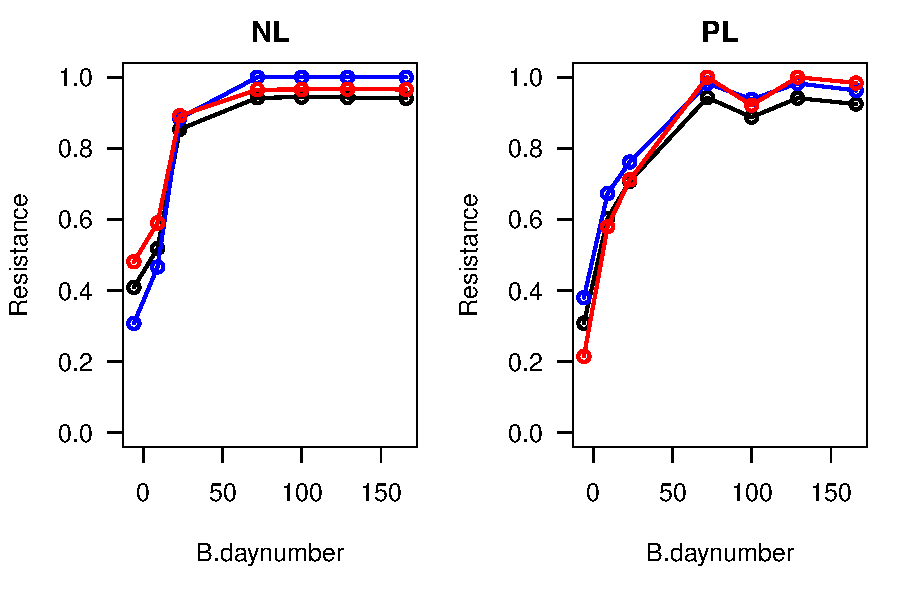
\includegraphics{analysis_ecoevostoich_files/figure-latex/unnamed-chunk-30-1.pdf}

\begin{verbatim}
##                   numDF denDF  F-value p-value
## (Intercept)           1    97 43.84393  <.0001
## B.trt                 1     4  1.45906  0.2936
## B.daynumber           6    97 14.27125  <.0001
## B.trt:B.daynumber     6    97  0.51041  0.7992
\end{verbatim}

\begin{longtable}[]{@{}ccccc@{}}
\toprule
\begin{minipage}[b]{0.29\columnwidth}\centering\strut
~
\strut\end{minipage} &
\begin{minipage}[b]{0.10\columnwidth}\centering\strut
numDF
\strut\end{minipage} &
\begin{minipage}[b]{0.10\columnwidth}\centering\strut
denDF
\strut\end{minipage} &
\begin{minipage}[b]{0.12\columnwidth}\centering\strut
F-value
\strut\end{minipage} &
\begin{minipage}[b]{0.12\columnwidth}\centering\strut
p-value
\strut\end{minipage}\tabularnewline
\midrule
\endhead
\begin{minipage}[t]{0.29\columnwidth}\centering\strut
\textbf{(Intercept)}
\strut\end{minipage} &
\begin{minipage}[t]{0.10\columnwidth}\centering\strut
1
\strut\end{minipage} &
\begin{minipage}[t]{0.10\columnwidth}\centering\strut
97
\strut\end{minipage} &
\begin{minipage}[t]{0.12\columnwidth}\centering\strut
2184
\strut\end{minipage} &
\begin{minipage}[t]{0.12\columnwidth}\centering\strut
0
\strut\end{minipage}\tabularnewline
\begin{minipage}[t]{0.29\columnwidth}\centering\strut
\textbf{B.trt}
\strut\end{minipage} &
\begin{minipage}[t]{0.10\columnwidth}\centering\strut
1
\strut\end{minipage} &
\begin{minipage}[t]{0.10\columnwidth}\centering\strut
4
\strut\end{minipage} &
\begin{minipage}[t]{0.12\columnwidth}\centering\strut
0.05589
\strut\end{minipage} &
\begin{minipage}[t]{0.12\columnwidth}\centering\strut
0.8247
\strut\end{minipage}\tabularnewline
\begin{minipage}[t]{0.29\columnwidth}\centering\strut
\textbf{B.daynumber}
\strut\end{minipage} &
\begin{minipage}[t]{0.10\columnwidth}\centering\strut
6
\strut\end{minipage} &
\begin{minipage}[t]{0.10\columnwidth}\centering\strut
97
\strut\end{minipage} &
\begin{minipage}[t]{0.12\columnwidth}\centering\strut
31.82
\strut\end{minipage} &
\begin{minipage}[t]{0.12\columnwidth}\centering\strut
0
\strut\end{minipage}\tabularnewline
\begin{minipage}[t]{0.29\columnwidth}\centering\strut
\textbf{B.trt:B.daynumber}
\strut\end{minipage} &
\begin{minipage}[t]{0.10\columnwidth}\centering\strut
6
\strut\end{minipage} &
\begin{minipage}[t]{0.10\columnwidth}\centering\strut
97
\strut\end{minipage} &
\begin{minipage}[t]{0.12\columnwidth}\centering\strut
0.5104
\strut\end{minipage} &
\begin{minipage}[t]{0.12\columnwidth}\centering\strut
0.7992
\strut\end{minipage}\tabularnewline
\bottomrule
\end{longtable}

\begin{longtable}[]{@{}ccccc@{}}
\toprule
\begin{minipage}[b]{0.29\columnwidth}\centering\strut
~
\strut\end{minipage} &
\begin{minipage}[b]{0.10\columnwidth}\centering\strut
numDF
\strut\end{minipage} &
\begin{minipage}[b]{0.10\columnwidth}\centering\strut
denDF
\strut\end{minipage} &
\begin{minipage}[b]{0.12\columnwidth}\centering\strut
F-value
\strut\end{minipage} &
\begin{minipage}[b]{0.12\columnwidth}\centering\strut
p-value
\strut\end{minipage}\tabularnewline
\midrule
\endhead
\begin{minipage}[t]{0.29\columnwidth}\centering\strut
\textbf{(Intercept)}
\strut\end{minipage} &
\begin{minipage}[t]{0.10\columnwidth}\centering\strut
1
\strut\end{minipage} &
\begin{minipage}[t]{0.10\columnwidth}\centering\strut
97
\strut\end{minipage} &
\begin{minipage}[t]{0.12\columnwidth}\centering\strut
1645
\strut\end{minipage} &
\begin{minipage}[t]{0.12\columnwidth}\centering\strut
0
\strut\end{minipage}\tabularnewline
\begin{minipage}[t]{0.29\columnwidth}\centering\strut
\textbf{B.trt}
\strut\end{minipage} &
\begin{minipage}[t]{0.10\columnwidth}\centering\strut
1
\strut\end{minipage} &
\begin{minipage}[t]{0.10\columnwidth}\centering\strut
4
\strut\end{minipage} &
\begin{minipage}[t]{0.12\columnwidth}\centering\strut
1.962
\strut\end{minipage} &
\begin{minipage}[t]{0.12\columnwidth}\centering\strut
0.2339
\strut\end{minipage}\tabularnewline
\begin{minipage}[t]{0.29\columnwidth}\centering\strut
\textbf{B.daynumber}
\strut\end{minipage} &
\begin{minipage}[t]{0.10\columnwidth}\centering\strut
6
\strut\end{minipage} &
\begin{minipage}[t]{0.10\columnwidth}\centering\strut
97
\strut\end{minipage} &
\begin{minipage}[t]{0.12\columnwidth}\centering\strut
27.78
\strut\end{minipage} &
\begin{minipage}[t]{0.12\columnwidth}\centering\strut
0
\strut\end{minipage}\tabularnewline
\begin{minipage}[t]{0.29\columnwidth}\centering\strut
\textbf{B.trt:B.daynumber}
\strut\end{minipage} &
\begin{minipage}[t]{0.10\columnwidth}\centering\strut
6
\strut\end{minipage} &
\begin{minipage}[t]{0.10\columnwidth}\centering\strut
97
\strut\end{minipage} &
\begin{minipage}[t]{0.12\columnwidth}\centering\strut
0.7992
\strut\end{minipage} &
\begin{minipage}[t]{0.12\columnwidth}\centering\strut
0.5729
\strut\end{minipage}\tabularnewline
\bottomrule
\end{longtable}

\begin{longtable}[]{@{}ccccc@{}}
\toprule
\begin{minipage}[b]{0.29\columnwidth}\centering\strut
~
\strut\end{minipage} &
\begin{minipage}[b]{0.10\columnwidth}\centering\strut
numDF
\strut\end{minipage} &
\begin{minipage}[b]{0.10\columnwidth}\centering\strut
denDF
\strut\end{minipage} &
\begin{minipage}[b]{0.12\columnwidth}\centering\strut
F-value
\strut\end{minipage} &
\begin{minipage}[b]{0.12\columnwidth}\centering\strut
p-value
\strut\end{minipage}\tabularnewline
\midrule
\endhead
\begin{minipage}[t]{0.29\columnwidth}\centering\strut
\textbf{(Intercept)}
\strut\end{minipage} &
\begin{minipage}[t]{0.10\columnwidth}\centering\strut
1
\strut\end{minipage} &
\begin{minipage}[t]{0.10\columnwidth}\centering\strut
97
\strut\end{minipage} &
\begin{minipage}[t]{0.12\columnwidth}\centering\strut
2394
\strut\end{minipage} &
\begin{minipage}[t]{0.12\columnwidth}\centering\strut
0
\strut\end{minipage}\tabularnewline
\begin{minipage}[t]{0.29\columnwidth}\centering\strut
\textbf{B.trt}
\strut\end{minipage} &
\begin{minipage}[t]{0.10\columnwidth}\centering\strut
1
\strut\end{minipage} &
\begin{minipage}[t]{0.10\columnwidth}\centering\strut
4
\strut\end{minipage} &
\begin{minipage}[t]{0.12\columnwidth}\centering\strut
0.4009
\strut\end{minipage} &
\begin{minipage}[t]{0.12\columnwidth}\centering\strut
0.561
\strut\end{minipage}\tabularnewline
\begin{minipage}[t]{0.29\columnwidth}\centering\strut
\textbf{B.daynumber}
\strut\end{minipage} &
\begin{minipage}[t]{0.10\columnwidth}\centering\strut
6
\strut\end{minipage} &
\begin{minipage}[t]{0.10\columnwidth}\centering\strut
97
\strut\end{minipage} &
\begin{minipage}[t]{0.12\columnwidth}\centering\strut
36.72
\strut\end{minipage} &
\begin{minipage}[t]{0.12\columnwidth}\centering\strut
0
\strut\end{minipage}\tabularnewline
\begin{minipage}[t]{0.29\columnwidth}\centering\strut
\textbf{B.trt:B.daynumber}
\strut\end{minipage} &
\begin{minipage}[t]{0.10\columnwidth}\centering\strut
6
\strut\end{minipage} &
\begin{minipage}[t]{0.10\columnwidth}\centering\strut
97
\strut\end{minipage} &
\begin{minipage}[t]{0.12\columnwidth}\centering\strut
1.557
\strut\end{minipage} &
\begin{minipage}[t]{0.12\columnwidth}\centering\strut
0.168
\strut\end{minipage}\tabularnewline
\bottomrule
\end{longtable}

\newpage

\subsubsection{Compositional resistance}\label{compositional-resistance}

\subsection{\texorpdfstring{\protect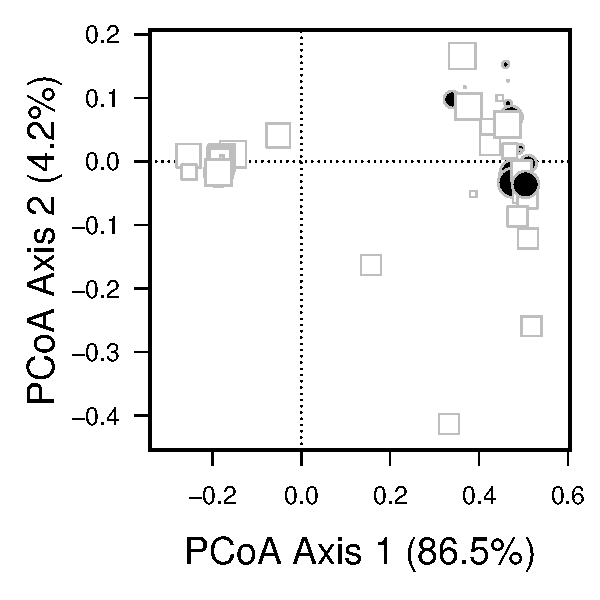
\includegraphics{analysis_ecoevostoich_files/figure-latex/unnamed-chunk-32-1.pdf}}{}}\label{section}

\begin{longtable}[]{@{}ccccccc@{}}
\toprule
~ & Df & SumsOfSqs & MeanSqs & F.Model & R2 &
Pr(\textgreater{}F)\tabularnewline
\midrule
\endhead
\textbf{Time} & 1 & 4.242 & 4.242 & 71.5 & 0.39 & 0.001\tabularnewline
\bottomrule
\end{longtable}

\textbf{Limitation} 1 0.03804 0.03804 0.6411 0.003496 0.017

**Time*Limitation** 1 0.07149 0.07149 1.205 0.006572 0.263

\begin{verbatim}
**Residuals**     110     6.527     0.05933     NA       0.6       NA   

  **Total**       113     10.88       NA        NA        1        NA   
\end{verbatim}

\begin{center}\rule{0.5\linewidth}{\linethickness}\end{center}

Table: Blocks: strata

\newpage

\subsection{Phage Host Range}\label{phage-host-range}

\subsubsection{global; sympatric vs.~allopatric host
range}\label{global-sympatric-vs.allopatric-host-range}

\newpage

\subsubsection{Compositional
infectivity}\label{compositional-infectivity}

\newpage

\subsection{Treatement level degree of
infection}\label{treatement-level-degree-of-infection}

\newpage

\section{Appendix}\label{appendix}

\subsection{R and packages}\label{r-and-packages}

All analyses were completed using R version 3.2.5 (2016-04-14)

\newpage

\subsection{References}\label{references}

\newpage

\subsection{Appendix}\label{appendix-1}

\subsubsection{Key term definitions}\label{key-term-definitions}

\begin{longtable}[]{@{}ccc@{}}
\toprule
\begin{minipage}[b]{0.24\columnwidth}\centering\strut
Word
\strut\end{minipage} &
\begin{minipage}[b]{0.19\columnwidth}\centering\strut
Abbreviation
\strut\end{minipage} &
\begin{minipage}[b]{0.15\columnwidth}\centering\strut
Definition
\strut\end{minipage}\tabularnewline
\midrule
\endhead
\begin{minipage}[t]{0.24\columnwidth}\centering\strut
Nitrogen
\strut\end{minipage} &
\begin{minipage}[t]{0.19\columnwidth}\centering\strut
N
\strut\end{minipage} &
\begin{minipage}[t]{0.15\columnwidth}\centering\strut
\strut\end{minipage}\tabularnewline
\begin{minipage}[t]{0.24\columnwidth}\centering\strut
Phosphorus
\strut\end{minipage} &
\begin{minipage}[t]{0.19\columnwidth}\centering\strut
P
\strut\end{minipage} &
\begin{minipage}[t]{0.15\columnwidth}\centering\strut
\strut\end{minipage}\tabularnewline
\begin{minipage}[t]{0.24\columnwidth}\centering\strut
Nitrogen Limited
\strut\end{minipage} &
\begin{minipage}[t]{0.19\columnwidth}\centering\strut
NL
\strut\end{minipage} &
\begin{minipage}[t]{0.15\columnwidth}\centering\strut
\strut\end{minipage}\tabularnewline
\begin{minipage}[t]{0.24\columnwidth}\centering\strut
Phosphorus Limited
\strut\end{minipage} &
\begin{minipage}[t]{0.19\columnwidth}\centering\strut
PL
\strut\end{minipage} &
\begin{minipage}[t]{0.15\columnwidth}\centering\strut
\strut\end{minipage}\tabularnewline
\begin{minipage}[t]{0.24\columnwidth}\centering\strut
chemostat
\strut\end{minipage} &
\begin{minipage}[t]{0.19\columnwidth}\centering\strut
cID
\strut\end{minipage} &
\begin{minipage}[t]{0.15\columnwidth}\centering\strut
\strut\end{minipage}\tabularnewline
\bottomrule
\end{longtable}

\end{document}
